\documentclass[12pt,italian]{report}
\usepackage{tesi}

\usepackage[a4paper]{geometry}		% Formato del foglio
\usepackage[italian]{babel}			% Supporto per l'italiano
\usepackage[utf8]{inputenc}			% Supporto per UTF-8
\usepackage[a-1b]{pdfx}				% File conforme allo standard PDF-A (obbligatorio per la consegna)

\usepackage{graphicx}				% Funzioni avanzate per le immagini
\usepackage{hologo}					% Bibtex logo with \hologo{BibTeX}
\usepackage{epsfig}				    % Permette immagini in EPS
\usepackage{xcolor}				    % Gestione avanzata dei colori
\usepackage{amssymb,amsmath,amsthm} % Simboli matematici
\usepackage{listings}				% Scrittura di codice
\usepackage{url}					% Visualizza e rendere interattii gli URL
\usepackage[pdfa]{hyperref}			% Rende interattivi i collegamenti interni
\usepackage{tikz}                   % Permette di disegnare inline
\usepackage{import}
\usepackage{float}
\usepackage{xstring}                % Permette di usare la funzione \IfInteger
\usepackage{array}                  % Permette di usare colonne "m" dentro table
\graphicspath{{immagini/}}

\usetikzlibrary{positioning}
\usetikzlibrary{calc}
\usetikzlibrary{shapes}

\newcommand{\GeneraSchemaPacchetto}[2]{{
\begin{tikzpicture}
    [
        box/.style={draw,rectangle,minimum width=\recminwidth, 
        minimum height=\rectangleheight, 
        outer sep=0pt, node distance=0pt}
    ]

    \def\rectangleheight{1cm}
    \def\recminwidth{2cm}

    \foreach \name/\size in {#1} {
        \node[box, label={below:\small \texttt{\size{} byte}}] (0) {\texttt{\name}};
    }    

    \foreach \name/\size [count=\i] in {#2}
    {
        \pgfmathtruncatemacro\prevposition{\i - 1}
        \node[box, right = 0pt of \prevposition,
            label={below:\small \texttt{\IfInteger{\size}{\size\ byte}{\size}}}
        ] (\i) {\texttt{\name}};
    }
\end{tikzpicture}
}}

\def\myCDL{Corso di Laurea magistrale in\\Informatica}

% TITOLO TESI:
\def\myTitle{Sicurezza Hardware in Ambienti Virtualizzati Tramite un Passthrough TEE tra QEMU e Linux}

% AUTORE:
\def\myName{Marco Cutecchia}
\def\myMat{Matr. Nr. 983828}

% RELATORE E CORRELATORE:
\def\myRefereeA{Prof. Danilo Bruschi}

% ANNO ACCADEMICO
\def\myYY{2022-2023}

% Il seguente comando introduce un elenco delle figure dopo l'indice (facoltativo)
%\figurespagetrue

% Il seguente comando introduce un elenco delle tabelle dopo l'indice (facoltativo)
%\tablespagetrue

\begin{document}

\frontespizio
\afterpreface

\chapter*{Sommario}
\addcontentsline{toc}{chapter}{Sommario}  
\label{cap:sommario}
L'aumento dei servizi che vengono richiesti dai moderni dispositivi di
computazione ha creato un quesito: l'aspetto di sicurezza è diventato più
importante di prima, ma con la maggiore complessità di tali sistemi aumenta
anche la superficie di attacco.
Rimuovere funzionalità dal sistema principale per renderlo più sicuro non
è accettabile, ma è possibile isolare i servizi critici dal punto di vista
della sicurezza in ambienti di computazione separati.

Questa è l'idea alla base dei \textit{Trusted Execution Environment(TEE)},
creare un ambiente di computazione nel processore isolato dal resto del
mondo non sicuro\cite{sabt2015tee}, e dedicato solamente a quei software
con requisiti di sicurezza stringenti.
Normalmente un software è completamente esposto a tutto il codice
presente nel sistema con un livello di privilegio superiore;
i TEE si separano da questa gerarchia isolando la propria memoria e i propri
dati dal resto del sistema affidandosi a una base hardware e software
molto piccola.

I TEE sono molto diffusi in ambito mobile, dove vengono utilizzati per
isolare servizi come l'autenticazione di dati biometrici\cite{androidbiometrics}
oppure la gestione di pagamenti digitali\cite{secure_payments}, ma inizia a esserci
un crescente interesse al loro
uso anche in ambito cloud\cite{confidential_computing_consortium} per
motivi di maggiore sicurezza,
normative dati e  per la possibilità di accertarsi che il software
in esecuzione sul server sia effettivamente quello che ci si aspetta.

Gli sforzi finora fatti in questo ambito sono stati rivolti verso permettere
ai clienti di portare i propri interi TEE; questa soluzione offre una grande
flessibilità ma implica anche uno sforzo significativo da parte del cliente
di gestire il proprio TEE, che per definizione è completamente inaccessibile
al vendor del cloud.

Le soluzioni oggi disponibili sul mercato sono esclusivamente per
l'architettura x86\_64 e implicano un lock-in rispetto le tecnologie
proprietarie di Intel e AMD.

Questa tesi si propone di studiare un modello alternativo dove il provider
di servizi cloud offre un TEE con dei servizi pre-installati offerti ai
clienti
Questo modello, seppur meno flessibile, è più semplice per il cliente e non
è in contrasto con il modello precedente. Questo offre un alternativa
ai clienti che non vogliono gestire il proprio TEE.
Inoltre, con la standardizzazione dell'interfaccia esterna TEE da parte di
dell'organizzazione GlobalPlatform\cite{gp2020clientapi}, è anche possibile
evitare il lock-in rispetto a un TEE specifico o a una
architettura in particolare.

Per dimostrare la fattibilità di questo modello abbiamo sviluppato un
prototipo estendendo l'hypervisor QEMU, scrivendo un driver Linux e
testando il tutto con il TEE open-source OP-TEE su piattaforma ARM.

\chapter{Introduzione}
\label{sec:introduzione}
I sistemi informatici moderni sono estremamente complessi e sono composti da
molti componenti diversi che interagiscono continuamente tra di loro.
Questa complessità può rendere difficile garantire che tali sistemi siano
sicuri e dunque privi di vulnerabilità.

Uno dei principali problemi è la difficoltà di testare e verificare
completamente la sicurezza di un sistema a causa del gran numero di
componenti e interfacce di comunicazione.
Ad esempio, un sistema potrebbe contenere al suo interno un componente che
singolarmente non ha vulnerabilità ma che potrebbe aprire una falla di
sicurezza quando combinato con un altro.
Dato l'incredibile numero di combinazioni possibili, è molto difficile
prevedere e valutare accuratamente il rischio di vulnerabilità di un sistema
in anticipo, in modo da implementare contromisure efficaci.

Inoltre i sistemi informatici sono in costante evoluzione, con
l'aggiunta di nuove funzionalità e capacità nel corso del tempo.
Ciò può rendere difficile mantenere la sicurezza di un sistema, poiché nuove
vulnerabilità potrebbero sorgere a causa di modifiche che all'apparenza non
avrebbero dovuto avere tale effetto.

In generale, più un sistema è semplice, più è facile testare e verificare
la sua sicurezza. 
Tuttavia, ridurre la complessità dei sistemi informatici moderni è un
obiettivo ambizioso, poiché una moltitudine di fattori, sia tecnici
sia economici, rende difficile attuare questo piano.

Una proposta alternativa e più realistica è quella data dai
\textit{Trusted Execution Environments} (TEE).
I TEE, come suggerisce il nome, sono ambienti sicuri in cui è possibile
eseguire del software. Date le caratteristiche dei TEE, dentro essi
generalmente si esegue solamente software con necessità di sicurezza
particolarmente stringenti.

L'idea di un TEE è quella di fornire all'interno del dispositivo
un secondo sistema isolato dall'altro; questo, essendo
indipendente, può implementare delle policy di sicurezza più
stringenti rispetto a quelle del sistema principale senza però dover
rinunciare a funzionalità.

Un TEE, tramite l'uso di tecniche crittografiche, hardware di supporto
e un approccio di sviluppo che prioritizza la sicurezza sopra tutti
gli altri aspetti, può offrire un grado di sicurezza molto più elevato
rispetto a quello offerto da un sistema tradizionale.

Anche se esiste una interfaccia di comunicazione con i TEE standardizzata,
a basso livello questi possono essere implementati in modi
significativamente diversi.
Un esempio di tali differenze sono
\textit{AMD Secure Encrypted Virtualization}, che permette di crittografare
la memoria di una macchina virtuale, e \textit{Secure Enclave}
di \textit{Apple}, un intero secondo computer integrato nel primo.
Questi non sono assolutamente gli unici approcci possibili,
in generale però è possibile dire che per implementare un TEE è necessario
di supporto hardware dedicato, questo perché il software da solo non è in
grado di potersi difendere da altro software quando questo ha i suoi
stessi privilegi.

\section{Cloud computing e sicurezza}
\label{sec:cloud}
Gli ultimi anni hanno visto un cambiamento radicale nel modo in cui
i produttori di software distribuiscono i loro prodotti
grazie alla affermazione del \textit{Cloud Computing}.

In passato, l'unico modo per offrire un servizio web era quello di
acquistare o affittare dei server, occupandosi della loro manutenzione
e prevedendo le loro capacità in base alle previsioni di
utilizzo.
Con il modello cloud nasce il concetto di
\textit{Infrastructure as a Service}, ovvero la possibilità di affittare
l'intera infrastruttura di rete necessaria per eseguire la propria applicazione
web e lasciare l'onere di mantenerla al provider cloud.

Il cloud computing è diventato estremamente popolare negli ultimi anni
per la sua capacità di offrire risorse flessibili a basso costo
anche a piccole e medie imprese.
Questo modello è redditizio sia per i fornitori che per gli utenti,
con i fornitori che possono offrire servizi a un costo inferiore grazie
alle economie di scala e gli utenti che possono ridurre i costi IT e
aumentare la loro agilità e competitività.

\bigbreak \noindent

Ovviamente questo modello porta non solo vantaggi, ma anche nuove sfide
in termini di sicurezza.
L'uso di questo modello comporta che i dati e il codice vengano spostati
su server remoti che non sono più in mano nostra.
Il controllo di questi server permette ai provider di ottimizzare al meglio
l'uso delle risorse fisiche disponibili e di offrire servizi a prezzi molto
convenienti, ma d'altro canto questo comporta una perdita del controllo
di cosa avviene al software durante l'esecuzione nei server e di 
chi può accedere ai dati oltre a loro.

Seppur sia lecito aspettarsi che i provider di servizi cloud siano onesti
e non vadano a sabotare i propri clienti, questa potrebbe non essere
una garanzia sufficiente per tutti.

Inoltre, il modello di cloud include un secondo attaccante: gli altri
clienti.
Il modo in cui i provider possono permettersi di offrire servizi di cloud
computing a prezzi convenienti è quello di condividere i server tra più
clienti; utilizzando delle macchine virtuali un server
può ospitare le applicazioni di più clienti allo stesso momento.

L'utilizzo della \textit{virtualizzazione} consente ai provider di isolare
i clienti tra di loro, di adattare
dinamicamente le risorse computazionali a loro disposizione e di trasferire
i loro dati e applicazioni da un server a un altro in qualsiasi
momento, in modo completamente trasparente ai clienti.
Ciò permette ai provider di ottimizzare l'utilizzo delle risorse
fisiche e di equilibrare il carico di lavoro tra i server.

Il processo di suddivisione di un server tra i vari clienti avviene tramite
l'utilizzo di un \textit{hypervisor}, un software che controlla la creazione
e la gestione delle macchine virtuali su un server fisico.
Tuttavia, l'utilizzo di un hypervisor rappresenta anche una minaccia per
la sicurezza poichè esso ha accesso e può modificare i dati in memoria
di tutte le macchine virtuali.
Pertanto, un attaccante che riuscesse ad eludere le protezioni
dell'hypervisor può potenzialmente manipolare i dati di tutti i clienti
che utilizzano quel server.

Trattare tutte le possibili problematiche in termini di sicurezza del
cloud computing non è lo scopo di questa tesi.
Quanto descritto finora è solo una delle molte sfide che il cloud computing
comporta, ma è sicuramente una delle più importanti data la sua elevata
posta in gioco.

\section{Motivazione della tesi}
\label{sec:motivazione}
I TEE sono stati sviluppati principalmente per gli ambienti mobili
poichè questi dispositivi sono diventati una componente sempre più
rilevante nella nostra vita quotidiana, rendendoli pertanto un
obiettivo sempre più allettante per i cyber criminali.
Oggi, i TEE sono presenti su quasi tutti i cellulari, dove vengono
usati per eseguire operazioni sensibili come, ad esempio, la gestione
della schermata di sblocco del telefono e l'inserimento di dati bancari
o, in generale, il trattamento di chiavi crittografiche e dati sensibili.
Tuttavia, il loro utilizzo non è limitato solo a questo ambito.

In particolare siamo interessati al loro utilizzo insieme ai modello di
computing cloud per proteggere i dati.
Parlando di protezione dati nel cloud possiamo far riferimento a tre
aspetti:
\begin{itemize}
    \item \textbf{Dati in transito}: i dati devono essere protetti durante
    il trasferimento tra i client e i server.
    \item \textbf{Dati in storage}: i dati devono essere protetti anche
    quando sono inattivi sul server.
    \item \textbf{Dati in memoria}: i dati devono essere protetti durante
    l'esecuzione del codice sul server.
\end{itemize}

Se per i primi due aspetti esistono soluzioni ben consolidate, come ad
esempio il protocollo HTTPS per la protezione dei dati in transito e
l'uso di dischi cifrati per la protezione dei dati in archiviazione,
per l'ultimo aspetto, ovvero la protezione dei dati e del codice in
memoria durante l'esecuzione, non esiste ancora una soluzione standard.

Per far fronte a questa sfida, è stata fondata il
Confidential Computing Consortium (CCC), un gruppo di aziende che si sono
unite per sviluppare e promuovere l'uso dei TEE in ambito cloud
allo scopo di diffondere quello che chiamano \textit{Confidential Computing}.

Il Confidential Computing protegge i dati in memoria eseguendo operazioni
su di essi solamente dentro enclavi sicure come i TEE, rendendoli
inaccessibili anche agli stessi sviluppatori dei software.
L'interesse per questo paradigma è in particolare dato da quelle organizzazioni
che gestiscono dati sensibili come informazioni personali, dati finanziari o
di salute, e che hanno dunque alti requisiti in termini di confidenzialità
e integrità dei dati.

Il supporto attualmente disponibile per il Confidential Computing è
limitato a server con piattaforme Intel o AMD, in alcuni casi con un
forte lock-in rispetto alla piattaforma scelta.

Con un interesse crescente nell'utilizzo di architetture diverse da x86\_64
in ambito server, diventa sempre più importante sviluppare un sistema che
consenta l'utilizzo dei TEE in modo indipendente dalla piattaforma
hardware sottostante e dal TEE stesso.
A questo scopo, gli sforzi di standardizzazione delle interfacce TEE da
parte di GlobalPlatform rappresentano un grande contributo.

\bigbreak \noindent

Lo scopo di questa tesi è quello di costituire il primo passo verso questo
obiettivo, ovvero sviluppare un canale di comunicazione tra una macchina
virtuale e un generico TEE, in modo completamente agnostico alla piattaforma
hardware sottostante e al codice in esecuzione dentro al TEE.

Il software sviluppato in questa tesi non vuole essere un prodotto finito,
ma un prototipo che dimostri la fattibilità del progetto e che permetta
di iniziare a discutere di come implementare un sistema completo.
A tale scopo abbiamo deciso di estendere l'hypervisor QEMU e il sistema
operativo Linux per permettere la comunicazione tra una macchina virtuale
gestita dal primo e un TEE collegato al secondo.

\section{Struttura della tesi}
\label{sec:struttura-tesi}
La tesi è strutturata in tre capitoli principali:
\begin{itemize}
    \item Nel \textbf{Capitolo \ref{chap:tee}} diamo una introduzione al
    concetto di Trusted Execution Environment, alle sua applicazioni
    e a vari concetti correlati.
    \item Nel \textbf{Capitolo \ref{chap:hardware-supporto-tee}} discutiamo
    brevemente di varie soluzioni hardware a supporto dei TEE, delle loro
    caratteristiche e alcune vulnerabilità scoperte al riguardo.
    \item Nel \textbf{Capitolo \ref{chap:passthrough-tee-qemu-linux}}
    finalmente discutiamo del progetto di questa tesi, ovvero la creazione
    di un canale di comunicazione tra una macchina virtuale e un TEE.
\end{itemize}

In aggiunta a questi capitoli troviamo due appendici \ref{app:faketee} e
\ref{app:impostazione-ambiente-sviluppo-testing} che, seppur non essenziali
per la comprensione della tesi,
possono essere utili per risolvere alcune questioni tecniche
nel caso si fosse interessati a riprodurre o continuare il nostro lavoro.

\chapter{Trusted Execution Environment}
\label{chap:tee}
Un \textit{Trusted Execution Environment} (TEE) è un'area protetta in un
dispositivo che consente di eseguire codice autenticato in modo
più sicuro e attendibile rispetto al resto del sistema.

Con l'aumento della connessione e vulnerabilità dei dispositivi agli
attacchi, i TEE stanno diventando sempre più importanti.
Essi forniscono un modo per proteggere i dati e le operazioni sensibili
dall'accesso o dalla modifica non autorizzate e possono
essere utilizzati per una vasta gamma di applicazioni
in molti ambiti, di cui parliamo in \ref{sec:applicazioni-tee}.

Con l'importanza crescente dei dispositivi mobili nella nostra
vita quotidiana, non sorprende che i TEE siano presenti su praticamente
tutti i cellulari, tramite la piattaforma \textit{TrustZone} di ARM.
Gli esempi di TEE in questo ambito sono numerosi, alcuni nomi noti sono
\textit{Samsung Knox}, \textit{Qualcomm QTEE}, \textit{Google Titan-M}
e \textit{Apple Secure Enclave}.

L'utilizzo dei TEE non è limitato al solo del mondo mobile,
ma sta diventando sempre più importante anche in ambito IoT, Desktop e Server.
Sul mercato si stanno vedendo sempre più soluzioni che permettono di 
eseguire software in un ambiente protetto anche su queste piattaforme.

In questo capitolo illustriamo le caratteristiche chiave dei TEE e come
possono essere utilizzati per migliorare la sicurezza e l'affidabilità di
vari tipi di dispositivi e sistemi.

\section{TEE conformi GlobalPlatform}
\label{sec:tee-conformi-globalplatform}
I Trusted Execution Environment sono la combinazione di hardware e software
specificatamente progettati per creare un ambiente di computazione protetto e sicuro.
Tuttavia, il termine "TEE" è piuttosto generico e viene utilizzato per
descrivere una vasta gamma di prodotti che possono avere garanzie di
sicurezza e dettagli di implementazione significativamente diversi.

La mancanza di una definizione comune e standardizzata dei TEE
può causare confusione tra i consumatori e rappresentare un ostacolo per
gli sviluppatori interessati a creare applicazioni che possono essere
eseguite su più TEE,
poichè devono gestire una vasta gamma di differenze nell'implementazione
nelle garanzie di sicurezza effettivamente offerte.

Per risolvere questi problemi, il consorzio GlobalPlatform pubblica
dei documenti di specifica per i TEE, oggi arrivati alla
versione 1.3 pubblicati nel 2020.
Questi standard forniscono un insieme comune di linee guida e requisiti per
la creazione di TEE progettati per essere interoperabili e sicuri.

Più nel dettaglio, tra queste specifiche troviamo una architettura
generica per i TEE, un profilo di sicurezza e delle interfacce per
programmatori che permettono lo sviluppo di applicazioni portabili tra TEE
diversi. 

Diverse aziende e organizzazioni hanno adottato questi standard
ed hanno adattato le loro soluzioni per essere conformi alla specifica
GlobalPlatform.
Seppur esistano ancora sul mercato soluzioni non conformi non è difficile
prevedere che nel breve futuro la maggior parte dei TEE lo saranno.

Pertanto, la discussione in questa tesi si concentrerà sui
TEE conformi GlobalPlatform.

\subsection{Architettura TEE}
\label{subsec:architettura-tee}

La specifica GlobalPlatform non detta una architettura particolare per i
TEE, ma offre comunque esempi che possono essere utili per comprendere
quali sono i componenti fondamentali di un TEE GlobalPlatform e come
questi componenti collaborano tra di loro.

\begin{figure}
    \centering
    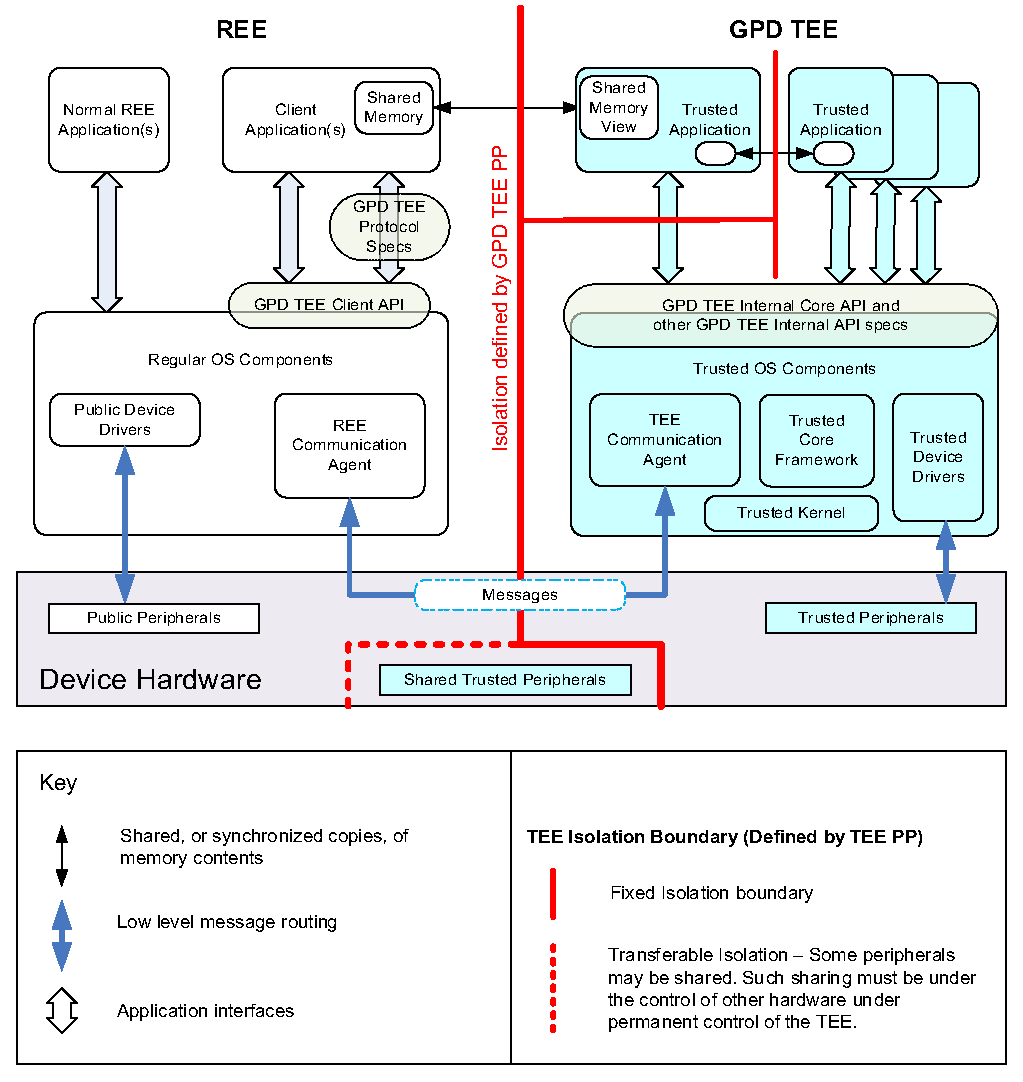
\includegraphics[width=1\textwidth]{immagini/tee-system-architecture}
    \caption{
        Architettura di un TEE conforme GlobalPlatform. 
        Da \textit{TEE System Architecture v1.3 (pag. 28)}
        \cite{gp2020systemarchitecture}
    }
    \label{fig:tee-system-architecture}
\end{figure}

In \figurename~\ref{fig:tee-system-architecture} è illustrata una possibile
architettura software di un sistema con un singolo TEE conforme
GlobalPlatform. Tuttavia, questa è solo una delle molte possibili
architetture e nulla vieta che un sistema possa avere più TEE, anche se
questo non è molto comune nella pratica.

In tale figura è possibile notare una barriera che divide il sistema in due
mondi: il mondo del \textit{Trusted Execution Environment} (TEE) a destra
e il mondo del \textit{Regular Execution Environment} (REE) a sinistra, cioè
il mondo a cui siamo abituati a lavorare con i sistemi operativi classici.

In entrambi i mondi troviamo un sistema operativo che gestisce le risorse
hardware e schedula l'esecuzione dei processi. Un programma in esecuzione
all'interno del TEE prende il nome di \textit{Trusted Application}(TA) e può
offrire servizi ad altre TA o alle applicazioni in esecuzione nel REE,
che prendono il nome di \textit{Client Application}(CA).

Le TA all'interno del TEE possono far uso del \textit{Trusted Core Framework},
che fornisce una interfaccia per operazioni comuni come il salvataggio
di file in modo sicuro, l'accesso al timer e altre funzionalità descritte
nella
\textit{Trusted Core Framework API Specification}\cite{gp2020internalapi}.
Questa interfaccia dovrebbe permettere di poter portare una TA su TEE diversi
senza doverne modificare il codice.

I due mondi non possono accedere direttamente all'altro, ma possono
comunicare solo tramite uno scambio di messaggi mediato dall'hardware.
Su questo meccanismo di comunicazione è possibile costruire meccanismi di
comunicazione a livello più alto, come ad esempio la condivisione di buffer
di memoria tra CA e TA.

\bigbreak \noindent

Il flusso di esecuzione tipico in un sistema con un TEE conforme GlobalPlatform
prevede che una Client Application richieda un servizio a
una Trusted Application tramite l'utilizzo della \textit{Client API}.
L'invio del primo messaggio apre una \textit{sessione} tra la CA e la TA, che
indica l'inizio di uno o più \textit{Function Invocation}.
Un messaggio di \textit{Function Invocation} contiene semplicemente un ID
che identifica la funzione da invocare e degli eventuali parametri;
il mapping tra ID e funzione è definito dalla \textit{Trusted Application}.
La TA esegue la funzione richiesta e risponde con un messaggio che contiene
l'esito dell'operazione ed eventuali dati di ritorno.

Queste chiamate sono sincrone, ma è possibile costruire delle chiamate
asincrone tramite un meccanismo di polling.

Entrambi i mondi del TEE e del REE dispongono di un proprio
\textit{Communication Agent}: questi 
hanno il compito d'inoltrare i messaggi tra CA e TA e, solo per il
\textit{TEE Communication Agent}, anche tra TA a TA.
Questi agenti possono assumere diverse forme, come processi, componenti
del sistema operativo o semplici librerie.
Seppur nello schema siano visti come solo due componenti, nella realtà
il loro ruolo può essere svolto usando più sotto-componenti.

\bigbreak

\noindent Infine, le periferiche hardware vengono suddivise in tre categorie:
\begin{itemize}
    \item \textit{Periferiche Fidate}: L'accesso a queste periferiche è
    esclusivamente consentito al TEE. Esempi di queste periferiche sono i
    sensori biometrici, come il lettore di impronte digitali. 
    \item \textit{Periferiche Fidate Condivise}: L'accesso a queste
    periferiche di default è consentito solamente al TEE, ma questo può
    decidere temporaneamente di condividere l'accesso con il REE. Esempi di
    queste periferiche sono il display e la tastiera.
    \item \textit{Periferiche Pubbliche}: L'accesso diretto a queste
    periferiche avviene dal REE, ma nulla impedisce a quest'ultimo di
    permettere l'accesso anche al TEE tramite un driver. Esempi di queste
    periferiche sono gli altoparlanti.
\end{itemize}

\subsection{Garanzie di sicurezza}
\label{subsec:garanzie-sicurezza}
I Trusted Execution Environment possono essere implementati modi diversi
tra di loro, di conseguenza non sarebbe corretto considerarli tutti
uguali dal punto di vista della sicurezza.
Per questo motivo, GlobalPlatform ha definito un set di proprietà che
tutti i TEE devono garantire, elencate nel
\textit{"Protection Profile"}\cite{gp2020protectionprofile}.
Un TEE, per essere certificato, deve garantire almeno queste proprietà, ma
può garantire anche proprietà aggiuntive.
Nonostante rimanga comunque sensata l'osservazione che non tutti i TEE
sono uguali, grazie al "Protection Profile" è possibile stabilire una
linea di base minima. 

Una analisi dettagliata di questi documenti è fuori dallo scopo di questa
tesi, ma in generale è possibile affermare che un TEE deve poter garantire
la proprietà di esecuzione isolata rispetto al REE e le proprietà d'integrità
e confidenzialità sia del codice sia degli assets generati da esso.

Le specifiche GlobalPlatform non restringono come queste proprietà devono
essere raggiunte, seppur proponga alcune soluzioni pratiche.
Tuttavia, esistono comunque degli aspetti comuni alla maggior parte dei
TEE, come ad esempio l'uso di supporto hardware per realizzare l'isolamento
oppure l'uso di firme digitali per garantire l'autenticità del codice.

\paragraph{Isolamento:}
% TODO: Leggi per davvero l'articolo di rushby
Per garantire la proprietà d'isolamento dal REE,
Sabt et al.\cite{sabt2015tee} nota
che tutti i TEE implementano un \textit{separation kernel}
\cite{rushby1981separationkernel}. 
Un \textit{separation kernel} è un componente hardware e/o software fidato che
separa il sistema in zone isolate che non possono
interagire direttamente tra di loro e gestisce le comunicazioni tra di esse.
% FIXME: Sembra tanto l'idea di microkernel, bisogna approfondire la differenza
L'idea non è nuova, infatti venne proposta da Rushby nel 1981 dove propose
di vedere ogni singola macchina come un sistema distribuito di componenti
indipendenti, in questo modo un errore in un singolo componente non avrebbe
compromesso l'intero sistema.

Questa idea viene ripresa nel mondo dei TEE allo scopo di ridurre la
potenziale superficie di attacco del sistema, in questo modo se un
attaccante riesce a compromettere un singolo componente gli altri rimangono
intatti, assumendo che il \textit{separation kernel} non venga anch'esso
compromesso.

Nei sistemi operativi oggi in uso, come Linux o Windows, la superficie di
attacco è molto vasta a causa dell'enorme quantità di hardware che devono
supportare e il numero elevato di servizi, anche non critici per la sicurezza,
che offrono ai programmi utente. 
Un attaccante che riesce a penetrare nel kernel ottiene il massimo livello di
controllo sulla macchina, diventa dunque sensata l'idea di separare quei
servizi importanti per la sicurezza e d'isolarli dal resto del sistema in
un ambiente sicuro.

Per questo motivo, è cruciale che il \textit{separation kernel} sia
il più semplice possibile, in modo dapoterlo verificare facilmente per
eventuali falle di sicurezza.
Seppur sia possibile avere molteplici TEE sullo stesso sistema, nella pratica
tutte le implementazioni si limitano a un singolo TEE, dunque il
"sistema distribuito" immaginato da Rushby è composto solamente da due
componenti, il TEE e il REE.

\paragraph{Integrità e autenticità:}
L'isolamento del TEE consente di garantire la protezione dei dati
in memoria durante l'esecuzione del codice.
Tuttavia, questi benefici possono essere annullati se l'integrità e
l'autenticità del codice e degli assets all'interno del TEE non vengono
garantite.
Un attaccante, infatti, potrebbe modificare il codice del TEE mentre il
dispositivo è spento, per poi riaccenderlo con del codice compromesso
che intenzionalmente rivela informazioni importanti.

Per questo motivo, è necessario garantire l'integrità e l'autenticità del
codice durante l'intero ciclo di vita del sistema.
Non è accettabile che queste proprietà non vengano assicurate fin dal primo
avvio o che vengano temporaneamente non garantite, pena l'impossibilità di
dichiarare il sistema come non compromesso.

Una soluzione per assicurare l'integrità e autenticità del codice consiste
nell'implementare un meccanismo di autenticazione basato su chiavi
private conosciute solamente da enti fidati.
Ogni software, prima di poter essere caricato dentro il TEE, deve
passare un processo di autenticazione che consiste nel confrontare un hash
calcolato sul codice con un hash firmato incluso con il software.
Questo hash deve essere firmato utilizzando una chiave privata la cui
corrispondente chiave pubblica è conosciuta dal TEE, in modo da poter
essere decrittato e confrontato con l'hash calcolato per
verificare che un ente fidato abbia approvato quella specifica versione
del software. 

L'unica eccezione a questa regola è il primissimo software mandato
in esecuzione sul sistema; questo non può essere autenticato perché non
è ancora presente alcun software in esecuzione che possa effettuare il
processo di verifica.
Per ovviare al problema, questo software viene caricato da una memoria
impossibile da sovrascrivere, come ad esempio le PROM, in modo da
poter assumere comunque che il software non sia stato compromesso.

\begin{figure}
\centering
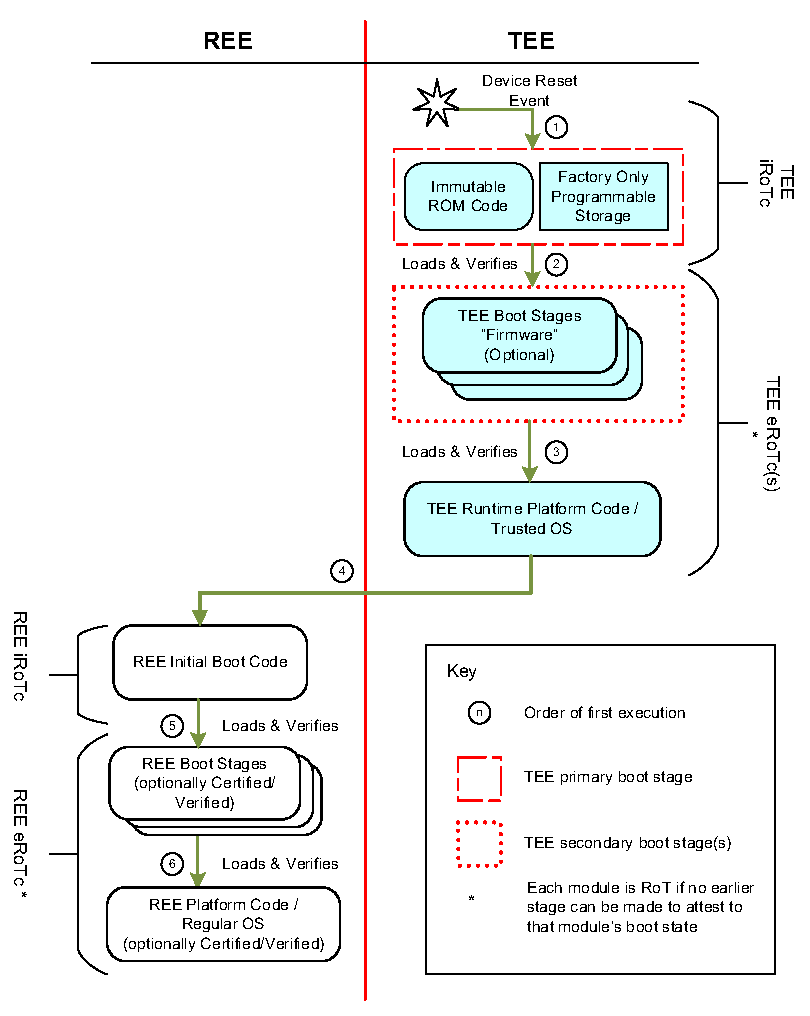
\includegraphics[width=0.8\textwidth]{immagini/tee-boot-sequence}
\caption{
    Sequenza di boot sicuro in un sistema con TEE. 
    Da \textit{GlobalPlatform TEE System Architecture pag. 73}
    \cite{gp2020systemarchitecture}
}
\end{figure}

Questo meccanismo di autenticazione è molto simile a quello utilizzato per
implementare il \textit{Secure Boot}; la differenza con quest'ultimo è che
nel \textit{Secure Boot} la catena di verifica del software termina con
l'avvio del sistema operativo, perché \textit{Secure Boot} si prefigge
di autenticare solamente processo di avvio del sistema operativo.
In un TEE, invece, vengono verificati anche i programmi
eseguiti al suo interno.

In entrambi i casi, però, è necessario che il firmware di un dispositivo
conosca le chiavi pubbliche per poter verificare la firma dei software
da caricare. Come queste chiavi vengano ottenute dal firmware è un dettaglio
implementativo, dunque altamente dipendente dal sistema.

\section{Applicazioni dei TEE}
\label{sec:applicazioni-tee}
I Trusted Execution Environment, con le loro maggiori garanzie d'integrità
e confidenzialità, non solo vengono utilizzati per aumentare la sicurezza
di applicazioni già esistenti, ma permettono lo sviluppo di nuove
applicazioni che non sarebbero possibili senza di essi.

Oggi i TEE sono largamente diffusi in ambito mobile, seppur non sempre
pubblicizzati, ma il loro utilizzo non è assolutamente limitato a tale ambito.
Le loro applicazioni sono molteplici, ma sfortunatamente la grande
maggioranza dei produttori di dispositivi non supportano
l'installazione di software aggiuntivo dentro il TEE dopo la
configurazione iniziale.

Questo però potrebbe cambiare nei prossimi anni: proposte come
\cite{kohlbrenner2020opentees} o \cite{penglai} aprono a più sviluppatori la
possibilità di implementare i propri TEE.
Inoltre, a seguito dell'adozione da più vendor degli standard GlobalPlatform,
e lo sviluppo di TEE open-source come OP-TEE, potremmo vedere nei prossimi
anni un uso più ampio di questa tecnologia e aperto a tutti.

\subsection{Secure Storage}
\label{subsec:secure-storage}
Una delle feature più comuni è l'uso dei TEE per la creazione del
\textit{Secure Storage}, una zona di memoria non volatile che possa rimanere
al sicuro anche quando il dispositivo è spento.

Questa area viene crittografata utilizzando una chiave conosciuta solamente
all'interno del TEE, la decifratura dei dati avviene solamente a seguito di
un controllo degli accessi da parte del TEE.

Un utilizzo molto comune di questa area sicura è il salvataggio di dati
come l'impronta digitale degli utenti, dati di accesso a servizi online
oppure la gestione delle chiavi crittografiche.
Molti sviluppatori di applicazioni mobile Android e iOS utilizzano
quest'ultima funzionalità grazie ad API che, se presenti, utilizzano delle
TA, come ad esempio "Keystore"\cite{androidkeystore} in Android.

Alcuni produttori, ad esempio AMD con il suo
\textit{Secure Processor}, utilizzano la
funzionalità di \textit{Secure Storage} per implementare un
\textit{Trusted Platform Module}(TPM) software\cite{amd2020ftpm}.
Questo è normalmente un chip dedicato al salvataggio sicuro di chiavi crittografiche
ed allo svolgimento di varie operazioni di crittografia; re-implementando
queste operazioni dentro un TEE è dunque possibile per i produttori risparmiare
il costo dell'hardware normalmente necessario per un chip TPM.

Il \textit{Secure Storage} viene utilizzato non solo per salvare
informazioni di cui vogliamo mantenere la confidenzialità ma anche per
informazioni per cui vogliamo assicurarci che un attaccante non possa
modificare a suo piacere.
Un esempio di quest ultimo caso è il numero i tentativi fatti per sbloccare
un telefono: questa non è una informazione privata, ma non vogliamo che un
attaccante possa modificare questo valore per darsi più tentativi ed evitare
che il dispositivo si blocchi.

% FIXME: È comunque vulnerabile a rollback attack

\subsection{Remote Attestation}
\label{subsec:remote-attestation}
Uno degli usi possibili dei TEE è quello di fornire un meccanismo di
\textit{Remote Attestation} (RA), ovvero la possibilità di verificare che
un dispositivo remoto stia effettivamente eseguendo il software che
ci aspettiamo.

Il problema dell'attestazione remota è stato ben studiato negli anni e
sono stati proposti diversi metodi per risolverlo con vari gradi di
sicurezza.
La sfida principale è quella d'impedire a un attaccante di falsificare
i risultati dell'attestazione, ovvero di far credere a un altro dispositivo
che il dispositivo remoto stia eseguendo un software che non sta veramente
eseguendo.

In questo ambito i TEE possono essere utilizzati per implementare un sistema
di attestazione remota in modo molto semplice.
Un TEE, dato che offre integrità del software al suo interno, può implementare
una piccola \textit{Trusted Application} che ha il compito di eseguire
i controlli di attestazione e generare un report firmato digitalmente.
La chiave privata utilizzata per firmare il report può essere generata al
momento della prima installazione del dispositivo, questa chiave non uscirà
mai dal TEE, garantendo dunque la sicurezza.

Il tipico caso d'uso della RA è quello di una rete aziendale dove si
vuole verificare che nessun computer sia stato manomesso
e che non stiano eseguendo software non autorizzato.
Migliorare la sicurezza di sistemi già esistenti non è il suo unico utilizzo:
la RA può diventare un elemento fondamentale per lo sviluppo di nuove
applicazioni innovative, come discuteremo più avanti in questo capitolo.

\subsection{Protezione dei diritti di autore}
\label{subsec:drm}
Con la diffusione dei servizi di streaming, i produttori di contenuti esitano
a mettere a disposizione dei loro contenuti perché temono che questi vengano
condivisi con utenti che non hanno pagato per accedervi.
Effettivamente sarebbe molto semplice per un utente utilizzare un software per
registrare il proprio schermo mentre guarda un film acquistato legalmente, per
poi condividerlo con altri utenti senza che questi debbano acquistarlo.

Una applicazione molto diffusa dei TEE è il loro utilizzo per la protezione
dei diritti di autore (DRM). 
Sistemi come Widevine\cite{widevine} e PlayReady\cite{playready} vengono
integrati dai distributori di contenuti digitali allo scopo di impedire, o
almeno ostacolare, l'estrazione dei contenuti e la loro condivisione.
Questi sistemi hanno diversi livelli di protezione dei contenuti in base alle
capacità hardware del dispositivo; i produttori di contenuti possono richiedere
che un dispositivo supporti almeno un certo livello di sicurezza prima di
concedergli l'accesso ai propri contenuti.
Per esempio, alcuni servizi di streaming basati su Widevine richiedono che il
dispositivo raggiunga il livello L1 per poter usufruire di contenuti in alta
definizione; questo livello è raggiungibile solamente se presente un TEE con
la TA Widevine installata.

Il livello più alto di protezione che questi sistemi offrono è basato sui TEE,
che vengono usati per molteplici scopi tra cui: il provisioning di una chiave
crittografica condivisa tra server e client, la verifica delle licenze digitali
online e offline, la decrittazione degli stream audio/video e per mostrare
a schermo il video senza che applicazioni esterne al TEE possano leggerne
i contenuti.
Per quest'ultima feature è necessario che sia presente un canale di
comunicazione fidato tra TEE e display, cioè che non dipenda dal REE, in modo
che un attaccante non possa leggere i pixel in chiaro che verranno mostrati poi
sullo schermo.

\subsection{Protezione dati nel Cloud}
\label{subsec:protezione-dati-cloud}
Il modello di computing cloud permette di sfruttare le risorse di calcolo
disponibili in maniera efficiente e scalabile, ma allo stesso tempo introduce
nuovi problemi di sicurezza.
Questo modello richiede di permettere al cloud provider di controllare la
nostra macchina per poterla gestire e monitorare; se da un lato questo solleva
gli sviluppatori dal dover occuparsi di gestire le macchine, dall'altro ciò
comporta un rischio di sicurezza.
Infatti, se il cloud provider è in grado di controllare la nostra macchina,
questo significa che può anche leggere i dati in memoria.

La situazione diventa ancora più problematica quando consideriamo che su
una singola macchina fisica i provider eseguono più macchine virtuali, ciascuna
di clienti diversi ma che condividono la stessa memoria fisica.
Ci sono stati molti esempi in passato di attaccanti che sono riusciti a eludere
le misure di sicurezza per isolare la propria VM dalle altre
\cite{vmescape1}\cite{vmescape2}\cite{vmescape3}.
Questi attaccanti avrebbero avuto la possibilità non solo di spiare le altre
VM dei clienti che hanno avuto la sfortuna di risiedere sullo stesso server in
quel momento, ma anche di manipolare il loro codice per i loro scopi.

Una organizzazione che dipende dal cloud e con particolari requisiti in
termini di sicurezza potrebbe dunque volere una sorta di garanzia che il
software che sta eseguendo sia quello che è stato consegnato al provider.
Questo è il problema della attestazione remota, per cui abbiamo già discusso
in \ref{subsec:remote-attestation} come i TEE possono aiutare.

Il Confidential Computing Consortium\cite{confidential_computing_consortium}
è un consorzio di grandi aziende nel mondo cloud che lavora a questo problema
e, che al momento, trova nei TEE il modo per risolverlo.
Lo scopo dell'organizzazione è proprio quello di supportare lo sviluppo
di strumenti open source per garantire la sicurezza dei dati in memoria.
Questo è un campo di ricerca molto attivo e con molti progetti in corso ma
ancora poche soluzioni concrete e implementate.

\subsection{Altre proposte}
\label{subsec:altre-proposte}
In letteratura sono state proposte diverse applicazioni dei TEE nelle più
svariate aree. Di seguito ne elenchiamo alcune per dare un'idea di come
possano essere utilizzati nelle applicazioni più disparate.

\bigbreak \noindent

In Javet, Anciaux et al.\cite{teeuses_edgeletcomputing} viene proposto di
utilizzare i TEE per realizzare un sistema di computazione "on the edge" sopra
"Opportunistic Networks"(OppNet), ovvero reti che sfruttano i
pattern di movimento degli utenti per creare reti temporanee.
In questo modello i TEE vengono usati per implementare un meccanismo di
attestazione remota per permettere ai dispositivi di verificare l'autenticità
dei dati ricevuti da altri dispositivi.

\bigbreak \noindent

Nel mondo blockchain sono state proposte diverse soluzioni per implementare
un sistema di consenso distribuito più efficiente utilizzando i TEE.
Per esempio, in \cite{teeuses_blockchainconsent} viene proposto di utilizzare
i TEE per implementare una serie di primitive sulla quale poi viene
costruito un algoritmo di consenso che richiede solo $O(n)$ scambi di messaggi
tra i nodi.

Un'altra proposta, sempre in questo mondo, cerca di migliorare l'efficienza
nell'esecuzione degli smart contract.
Gli smart contract sono dei programmi salvati sulla blockchain e che vengono
eseguiti in modo automatico da tutti i nodi quando delle condizioni vengono
soddisfatte.
In \cite{teeuses_smartcontract} viene proposto di eseguire gli smart contract
direttamente sui TEE dei nodi e di far verificare la correttezza del risultato
dall'esterno tramite il meccanismo di attestazione remota.

\bigbreak \noindent

Infine in \cite{teeuses_vehicles} viene proposto di utilizzare i TEE per
implementare un protocollo per il coordinamento di veicoli a guida
autonoma in modalità Vehicle-to-Vehicle (V2V).
L'utilizzo dei TEE in questo protocollo permette di evitare che i veicoli
possano essere manipolati da attaccanti esterni e che i dati vengano
intercettati e utilizzati per tracciare gli spostamenti delle persone. 

\section{Questioni etiche nell'uso dei TEE}
\label{sec:etica-tee}
% FIXME: Fa schifo sta sezione
I Trusted Execution Environment introducono una serie di questioni etiche.
In letteratura nessuno ha ancora affrontato queste questioni rispetto ai TEE,
esistono però articoli riguardanti il concetto di \textit{Trusted Computing},
che è una tecnologia che condivide alcuni aspetti con i TEE, in particolare
l'idea che un sistema debba verificare a priori l'autenticità e l'integrità
del software prima di eseguirlo.

I TEE tolgono il pieno controllo della macchina all'utente, in quanto una
zona del sistema viene blindata e l'accesso ad essa è consentito solamente
a parti autorizzate da chi può firmare le Trusted Application.
Un singolo software insicuro può compromettere permanentemente la sicurezza
di un TEE, e quindi di tutto il sistema; non è possibile dunque permettere
l'esecuzione di qualunque software al suo interno.
Questa responsabilità è troppo grande per essere affidata a un utente,
che può dunque soltanto eseguire software che è stato approvato da un
ente fidato (ad esempio il produttore del dispositivo).
Stallman, in \textit{"Can You Trust Your Computer?"}\cite{stallman2021tpm},
osserva che le tecnologie di Trusted Computing, ma anche i TEE, non solo
difendono il sistema da attacchi esterni, ma anche dall'utente stesso
del sistema.

La maggior parte dei produttori non rilascia il codice sorgente
dei propri TEE; ma anche se così fosse, ciò non garantisce che il codice
in esecuzione sia quello rilasciato, in quanto il TEE installato sul
dispositivo potrebbe essere stato modificato prima dell'installazione.
Non è neanche possibile per un utente ricompilare il TEE e installarlo
sul proprio dispositivo dato che, per design, la chiave per firmare
il TEE non può essere estratta dal dispositivo.
Di conseguenza, il rischio è che un produttore possa preinstallare del
software sgradito all'utente sul suo dispositivo, e che questo software
possa essere eseguito in un TEE, senza che l'utente possa fare nulla
e alla sua insaputa.

Un aspetto interessante, ma sfortunatamente non ancora esplorato
in letteratura, è come permettere agli utilizzatori di un TEE di
verificarne il codice senza comprometterne la sicurezza.
Seppur questo non risolva la questione della perdita di controllo sulla
propria macchina, almeno permetterebbe di avere un'idea di cosa stia
eseguendo il TEE.

Un altro aspetto da considerare è che i TEE permettono di implementare
applicazioni che possono facilitare l'instaurazione di un monopolio
o anche di dubbia moralità.
Ad esempio, tramite l'uso di chiavi crittografiche generate dentro
il TEE, è possibile sviluppare un software di videoscrittura che
rende apribili i documenti solamente tramite esso, rendendo impossibile
qualunque sforzo di reverse-engineering. 
Oppure, tramite i TEE è possibile sviluppare un software di messaggistica
dove un capo in remoto può decidere se rendere inaccessibili certi messaggi
inviati in precedenza, permettendo di cancellare prove compromettenti.

\chapter{Hardware a supporto dei TEE}
\label{chap:hardware-supporto-tee}
Un TEE non può garantire le sue proprietà di sicurezza se non è supportato
da adeguato hardware, in particolare per quanto riguarda la proprietà di
isolamento dal resto del sistema considerato "non sicuro".

Non esiste una soluzione univoca per permettere che un TEE implementi
queste proprietà; pertanto, in questo capitolo verranno esplorate
brevemente alcune delle proposte hardware disponibili sul mercato.

\section{ARM TrustZone}
\label{sec:arm-trustzone}
ARM TrustZone\cite{trustzone} è una tecnologia introdotta da ARM nel 2004 che
fornisce un insieme di funzionalità hardware per la sicurezza
dei processori con profilo A (Application) e recentemente
anche M (Microcontroller).
Alcuni esempi di TEE famosi che utilizzano TrustZone sono
\textit{Samsung Knox}, \textit{Qualcomm QTEE} e \textit{OP-TEE}.

L'idea alla base di TrustZone è quella di virtualizzare il
processore, che può trovarsi in uno dei due stati:
\emph{"Secure"} o \emph{"Non-secure"}.
Questi stati possono accedere a memoria e periferiche diverse
e sono isolati l'uno dall'altro tramite sistemi di protezione
hardware.
Le modalità di privilegio di ARM, che vanno da EL2 (più alto)
a EL0 (più basso), vengono estese con le modalità
S-EL0, S-EL1, EL3.
A partire da ARMv8.4-A, TrustZone supporta anche il livello
di privilegio S-EL2, ma rimane una feature opzionale.

\begin{figure}[h]
    \centering
    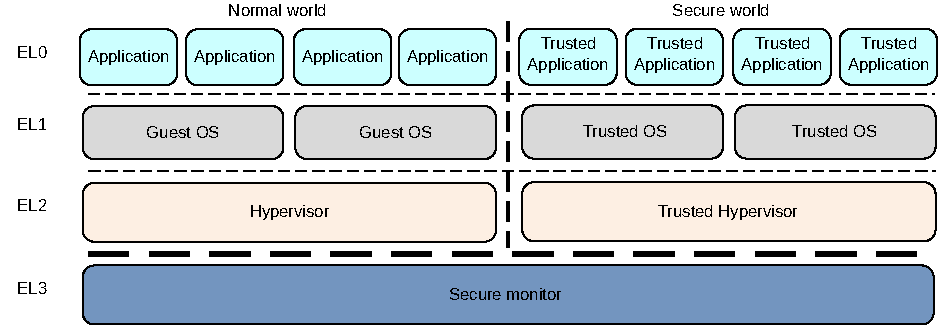
\includegraphics[width=0.8\textwidth]{immagini/aarch64-exception-levels}
    \caption{
        Livelli di privilegio di ARM TrustZone e il software
        che solitamente viene eseguito al loro interno.
        Adattato da
        \textit{"ARM Cortex-A Series Programmer's Guide for ARMv8-A"}
        \cite{arm_programmers_manual}
    }
    \label{fig:arm-exception-levels}
\end{figure}

Il livello di privilegio EL3 è il livello più alto e viene utilizzato
dal firmware per configurare il sistema e gestire la transizione
tra il mondo \emph{Secure} e quello \emph{Non-secure} in TrustZone.
In questo contesto, il livello EL3 rappresenta il
\emph{Separation Kernel} descritto in precedenza.

Il processore si avvia in questo livello eseguendo il firmware da una ROM.
Tra i compiti di questo firmware c'è quello di partizionare la memoria in
"memoria sicura" e "memoria non sicura", e di configurare quali
periferiche sono accessibili in modalità \emph{Secure} e quali
in modalità \emph{Non-secure}.
Le periferiche hanno accesso a un bit extra sul bus dati che
indica se il processore è in modalità \emph{Secure} o
\emph{Non-secure}.
Tramite questo bit, dato che su ARM le periferiche comunicano tramite MMIO,
una periferica potrebbe decidere se rifiutarsi di essere utilizzato
in modalità \emph{Non-secure}. 

Il firmware deve anche configurare un handler per l'istruzione
\textit{Secure Monitor Call}(\texttt{smc}).
Questa istruzione opera in modo simile a una \textit{system/hypervisor call}:
quando chiamata con un codice numerico specifico, cambia il livello
di privilegio a EL3 e passa il controllo a un handler impostato dal firmware.
Questo handler è impostato nella tabella degli interrupt del processore.

L'uso di questa istruzione permette di implementare il passaggio
di messaggi tra il mondo \emph{Secure} e quello \emph{Non-secure}, ed è
anche il modo usato da OP-TEE.

Il processore in modalità \emph{Secure} può accedere a tutta la memoria
e le periferiche, mentre in modalità \emph{Non-secure} può accedere
solamente a memoria e periferiche segnate come non sicure.
La decisione di quali periferiche e la zona di memoria sicura può essere
definita dal firmware a runtime oppure essere prefissata dal produttore
dell'hardware.

\medbreak \noindent

Il firmware in EL3 ha anche il compito di caricare i sistemi operativi
del mondo \emph{Secure} e \emph{Non-secure}.

TrustZone non definisce alcun sistema per verificare l'integrità del codice
all'avvio; questo problema è invece lasciato ai produttori di dispositivi.
Una soluzione popolare è quella di generare una coppia di chiavi pubblica
e privata, e di stampare l'hash della chiave pubblica nel chip e renderla
accessibile in modalità \emph{Secure} tramite un registro dedicato.

Il codice da caricare viene impacchettato insieme a un certificato
contenente l'hash del codice, una firma e la chiave pubblica utilizzata
per firmare l'hash.
Il firmware può calcolare l'hash della chiave letta dal codice, confrontarla
con quella dal registro locale e, se corrispondono, utilizzare la
chiave pubblica per verificare la firma dell'hash del codice.

Se la verifica fallisce, il firmware può decidere di continuare il boot
del mondo \emph{Non-Secure}, rendendo inutilizzabili i servizi del mondo
\emph{Secure}, o addinon caricare il codice
e rendere inaccessibile la modalità \emph{Secure}

\section{Intel SGX}
\label{sec:intel-sgx}
Intel Software Guard Extensions (SGX) è una estensione
dell'architettura x86\_64 introdotta nel 2015 con i processori
Intel Core di sesta generazione.

Intel SGX permette di creare delle \textit{enclavi}, aree di
memoria private e crittografate di piccole dimensioni.
L'accesso ai dati dentro una enclave consentito solamente se
il processore è entrato dentro di esse tramite i nuovi meccanismi
introdotti da SGX, ad esempio l'istruzione \texttt{EENTER}.

SGX implementa un approccio radicalmente diverso rispetto a TrustZone, e
non necessità un sistema operativo separato per il TEE, seppur sia comunque
possibile utilizzarlo in questo modo.
Questo approccio permette d'integrarsi in ambienti cloud senza difficoltà,
infatti SGX è una delle poche soluzioni hardware oggi disponibili
per utilizzare un TEE su tali piattaforme.

Le enclavi sono eseguibili solamente in \textit{protected mode}
a livello di privilegio $3$(il più basso) e possono essere create
solamente dal sistema operativo, per conto suo oppure di un'applicazione.

Constan e Devadas in \cite{sgx_explained} offrono una descrizione molto
dettagliata di come funziona SGX:
all'avvio della macchina, il sistema operativo può designare una zona
di memoria contigua come \textit{Processor Reserved Memory} (PRM) impostando
due registri e con una dimensione massima di 128MB e potenza di $2$.

Questa zona di memoria viene suddivisa in sottosezioni, tra cui troviamo
la \textit{Enclave Page Cache}(EPC) e la
\textit{Enclave Page Cache Map}(EPMC).
La EPC è un pool di memoria suddiviso in pagine di 4KB che possono essere
assegnate a enclavi oppure utilizzate per contenere strutture dati di
supporto a SGX.
L'accesso a questa memoria è consentito solamente all'enclave a cui è
assegnata la pagina corrispondente, altrimenti il processore leggerà tutti
i bit a $1$.
La EPMC è una tabella utilizzata da SGX per tracciare le pagine della EPC
a quale enclave appartengono ed è inaccessibile a chiunque, indipendentemente
dal livello di privilegio.

La creazione di una enclave è compito del sistema operativo e
avviene in tre fasi:
inizialmente il SO seleziona una pagina libera della EPC in cui scrive una
struttura dati chiamata \textit{SGX Enclave Control Structure}(SECS)
contenente diversi parametri riguardo all'enclave. 
Il sistema operativo chiama \texttt{ECREATE} passando questa pagina, che
diventerà poi inaccessibile a chiunque dato che SGX la utilizzerà per
salvare metadati riguardo l'enclave.
L'indirizzo virtuale della SECS diventerà un identificatore per l'enclave.

Una volta create l'enclave, il sistema operativo deve assegnargli memoria
e copiare al suo interno i dati iniziali.
Per fare questo utilizza l'istruzione \texttt{EADD} passando
l'indirizzo virtuale a una struttura dati chiamata
\textit{SGX Enclave Page Information}(EPI) che contiene
informazioni riguardo la pagina di EPC da utilizzare per l'enclave
e, opzionalmente, se copiare al suo interno i dati da un'altra pagina
di memoria.

Infine è necessario inizializzare l'enclave prima di poter eseguire
il codice al suo interno.
Per fare ciò il sistema operativo chiama \texttt{EINIT} passando
un \textit{Init Token Structure}. Questo token può essere generato grazie
a una enclave speciale fornita da Intel chiamata \textit{Launch Enclave}
che può essere approvata localmente dalle CPU SGX perchè firmata con una
chiave installata nell'hardware.

La Launch Enclave si appoggia a un servizio remoto alla quale
gli sviluppatori possono iscriversi, previa verifica di Intel, per caricare
un proprio certificato pubblico.
Una enclave deve essere distribuita con un \textit{Measurement Hash}(MH)
firmato con tale certificato.
Un MH è un hash generato da SGX che rappresenta lo stato di una enclave appena
prima che questa possa eseguire la sua prima istruzione, la Launch Enclave
dunque utilizza il MH misurato, il MH incluso firmato e il
certificato pubblico per verificare l'integrità della enclave e generare il
token d'inizializzazione.

\medbreak \noindent

Intel SGX è implementato quasi interamente in microcodice: 
grazie a questa scelta anche se SGX nel tempo ha sofferto
di diverse vulnerabilità, Intel ha potuto risolverle rilasciando
aggiornamenti puramente software.

A partire dal 2021, Intel SGX è stato deprecato sui processori Intel Core
di undicesima e dodicesima generazione\cite{sgx_deprecation}.
Intel non ha rilasciato spiegazioni, ma continua lo sviluppo di SGX per
i processori Intel Xeon, comunemente usati sui server. 

\section{AMD Secure Encrypted Virtualization}
\label{sec:amd-sev}
AMD Secure Encrypted Virtualization (SEV) è una estensione dell'architettura
x86\_64 introdotta nel 2017\cite{sev} con la prima serie
di processori Epyc.

AMD SEV permette di crittografare la memoria di una macchina virtuale in
modo che, anche se l'hypervisor viene compromesso, non sia possibile per
l'attaccante leggere i dati della macchina virtuale.
L'idea di SEV è simile a quella di SGX, ma invece di creare delle enclavi
il concetto è applicato alle macchine virtuali.
AMD SEV è una soluzione mirata per le esigenze dei provider cloud,
infatti include inoltre meccanismi per permettere la migrazione di VM
tra host.

Alla base del funzionamento di SEV sono un chip AES-128 installato sui
bus di memoria, che si occupa della cifratura dei dati in memoria,
e un processore ARM installato sulla scheda madre chiamato 
\textit{Secure Processor}(SP)
\footnote{
    Precedentemente chiamato \textit{Platform Security Processor} (PSP).
}(SP).
Questo processore aggiunto esegue un sistema operativo proprietario che
ha vari compiti, come ad esempio generare e gestire le chiavi crittografiche
usate per crittografare la memoria delle VM.

Il SP è in grado di generare un report di attestazione per ogni VM
in esecuzione, questo permette di implementare un sistema di
attestazione remota.
Questi report vengono inviati ai clienti, che vogliono aver modo di
verificare che le VM in esecuzione su un server siano state create
da un'immagine verificata e sono in esecuzione nell'ambiente desiderato.
Un report di attestazione contiene informazioni tra cui un hash dell'immagine
della VM caricata dall'hypervisor, le tabelle di mapping della memoria
impostate inizialmente per la VM, funzionalità di sicurezza abilitate
sul sistema e versioni dei componenti hardware.
Questo report viene firmato utilizzando una chiave privata installata nel
processore, estraibile (in teoria) solamente con tecniche distruttive e
che richiedono accesso fisico.
I clienti possono quindi verificare che il report sia stato firmato da
una chiave privata di un processore AMD utilizzando il certificato pubblico
di AMD disponibile online. 

\medbreak

Successivamente AMD ha rilasciato una versione aggiornata di SEV, chiamata
SEV-ES (Encrypted State)\cite{sev_es}. SEV salva i registri
di una VM in chiaro dopo un context switch con l'hypervisor, questo è
stato ritenuto un problema di sicurezza e dunque SEV-ES ha introdotto la
crittografia anche degli stati dei registri.

SEV-SNP (Secure Nested Paging)\cite{sev_snp}, rilasciata nel 2021
con la terza serie di processori Epyc, è l'ultima versione di SEV
disponibile al momento.
SEV-SNP include protezioni aggiuntive verso
attacchi \textit{replay}, attacchi che sfruttavano mapping di memoria
intenzionalmente inconsistenti per bypassare alcune protezioni di SEV
e delle correzioni generali a vulnerabilità scoperte nelle versioni 
precedenti.

\section{Processori dedicati}
\label{sec:processori-dedicati}
Una soluzione possibile per implementare un TEE è quella di utilizzare
un intero secondo sistema, collegato solamente alle periferiche fidate.
Chiaramente integrare un secondo \textit{System on a Chip}(SoC) dentro
a un dispositivo è una soluzione più costosa, ma possibile, particolarmente
in dispositivi di fascia premium.

\bigbreak \noindent

Apple, a partire dall'iPhone 5, include nei propri telefoni un sottosistema
integrato nel processore che prende il nome di
\textit{Secure Enclave}.
Questo è un SoC che esegue una versione modificata del
microkernel L4\cite{secure_enclave}.
Il chip \textit{Secure Enclave} è collegato solamente ad alcuni
acceleratori crittografici e a un bus I2C per salvare dati in una zona di
memoria non volatile dedicata.
Il suo scopo è quello di mantenere i dati
degli utenti al sicuro in caso di compromissione del processore principale
e implementare servizi come \textit{Touch ID} e \textit{Apple Pay}.

\bigbreak \noindent
Anche Google implementa una soluzione simile per i suoi telefoni Pixel.
I telefoni Pixel 6 e Pixel 6 Pro integrano il processore
\textit{Google Tensor}, un processore proprietario basato su ARM e che
utilizza TrustZone per implementare un TEE.
Affiancato a questo chip, ne troviamo un altro chiamato \textit{Titan M2}:
questo è un \textit{System on a Chip} proprietario RISC-V dedicato a
scopi simili a quelli di \textit{Secure Enclave}.   
Nei propri telefoni, Google utilizza l'area TrustZone solamente come
intermezzo per la comunicazione con il chip \textit{Titan M2} e per
implementare il meccanismo di \textit{Secure Boot} per il mondo
non sicuro.

\bigbreak \noindent

Ad oggi non sono stati segnalati attacchi alla \textit{Secure Enclave},
mentre è stato segnalato un singolo attacco\cite{attack_titanM} a
\textit{Titan M}.

\section{TEE RISC-V}
\label{sec:risc-v}
RISC-V è un Instruction Set Architecture(ISA) open source sviluppato
dalla RISC-V Foundation, una organizzazione senza scopo di lucro.
Sviluppare hardware basato su RISC-V è gratuito e non richiede alcuna
licenza, nasce per essere estensibile e inoltre gode di un buon supporto
tramite toolchain e sistemi operativi.
Questo ISA è molto interessante per i produttori di dispositivi perché
permette loro di sviluppare hardware adattato per le loro esigenze,
senza dover pagare licenze o scrivere completamente da zero un
completo stack software.

Queste caratteristiche hanno reso RISC-V un mondo dove diversi progetti
collegati all'ambito TEE stanno nascendo.
Molti di questi progetti si basano sull'estensione
\textit{Physical Memory Protection}(PMP), che permette di definire un
numero variabile(ma limitato dall'hardware) di aree di memoria fisica
protette da accessi non autorizzati.
Il funzionamento è simile a quello di SGX o TrustZone, senza però limiti
alla memoria delle enclavi e con la possibilità di configurare le enclavi.

Visto che l'interesse verso RISC-V è dato dalla possibilità di adattare
l'hardware a specifiche esigenze, non esiste un'implementazione standard
di un TEE RISC-V ma esistono dei progetti che permettono di costruire
dei TEE RISC-V integrabili nei propri design,
ad esempio Keystone\cite{keystone} e Penglai\cite{penglai}.

\section{Vulnerabilità comuni}
\label{sec:vulnerabilita-comuni}
I TEE sono progettati per essere sicuri, ma un famoso mantra dice che
\textit{"la sicurezza assoluta non esiste"}, e questo vale anche per i TEE.
Seppur i TEE offrano un livello di sicurezza molto elevato, sono stati
dimostrati in passato diversi attacchi che permettono di bypassare
le protezioni offerte da questi sistemi.

Il software dei TEE può essere aggiornato per risolvere questi problemi,
mentre gli attacchi hardware sono più difficili da risolvere.
Alcuni attacchi hardware possono essere risolti con aggiornamenti del
microcodice della CPU, ma questo non è sempre possibile e in tali casi
è necessario cambiare hardware. 

\medbreak
Un primo vettore di attacco è il software in esecuzione dentro il TEE:
vulnerabilità classiche come \textit{buffer overflow}, \textit{use after free}
o la mancata validazione degli input possono compromettere la sicurezza
dell'intero sistema.
Questi attacchi non sono dipendenti dall'hardware di supporto al TEE,
è possibile infatti trovare vulnerabilità simili anche in TEE che fanno
uso di hardware molto diversi tra loro.

Un esempio di attacco di questo tipo è stato segnalato nel 2022 verso
\textit{Titan M}\cite{attack_titanM}, il chip proprietario di Google
per i suoi telefoni Pixel.
Una vulnerabilità in una procedura di copia dati da un buffer temporaneo
ha permesso di scrivere un singolo byte a un indirizzo qualsiasi in memoria
sicura; tramite essa è stato possibile effettuare un attacco
di tipo \textit{ROP}\footnote{Return Oriented Programming}
ed estrarre informazioni private del TEE.

Le soluzioni a questo problema sono le stesse di qualsiasi altro software:
una progettazione tenendo conto della sicurezza fin dall'inizio, 
l'impiego di processi di code-review, l'uso di linguaggi di programmazione
\textit{memory safe}, e l'uso di strumenti di fuzzing, verifica formale e
analisi statica per trovare bug in anticipo sono tutte buone pratiche per
la sicurezza del software.

\bigbreak \noindent
Per molte soluzioni hardware la gestione della cache è stata
un punto dolente: sia su TrustZone, sia su SGX e sia su SEV
è stato possibile bypassare le protezioni offerte da questi sistemi
grazie a essa.
La gestione della cache in modo sicuro è un problema molto complesso,
che viene ulteriormente complicato dalla presenza dei TEE dato che
diventa necessario separare le linee di cache per la memoria del TEE
e per quella del REE.

Attacchi \textit{timing-based} sono stati dimostrati su TrustZone e SGX,
permettendo di estrarre dati privati dalla memoria del TEE e, in almeno
un caso, anche di scrivere dati nella memoria sicura.
Per esempio, \textit{CacheZoom}\cite{cachezoom} e
\textit{ARMageddon}\cite{armageddon} hanno permesso di estrarre dati
dalla memoria sicura, rispettivamente su Intel SGX e ARM TrustZone,
tramite attacchi alla cache di tipo \textit{Prime+Probe},
\textit{Flush+Reload} e altro.

Su ARM TrustZone, Guanciale et al.\cite{aliasdriven} hanno dimostrato
che, creando molteplici mapping virtuali allo stesso indirizzo fisico,
ma impostando politiche di caching incoerenti, è possibile non solo
leggere dati dalla memoria sicura, ma anche scrivere dati in alcuni casi.

Su AMD SEV, Mengyuan et all\cite{sev_tlb_poisoning} hanno trovato diverse
vulnerabilità nella gestione del \textit{Translation Lookaside Buffer},
riuscendo non solo a leggere dati dalla memoria sicura di una VM, ma anche
a forzarla a eseguire una singola istruzione arbitraria.

Inoltre, seppur non sia una vulnerabilità del TEE, è stato
dimostrato che la gestione separata della cache tra TEE e REE
può essere utilizzata da rootkit nel REE per nascondersi da strumenti
di analisi.
Ad esempio, CacheKit\cite{cachekit} è un rootkit per sistemi Linux
su piattaforme ARM con TrustZone che inietta il proprio codice nella
cache senza però essere presente in memoria.
CacheKit sfrutta le linee di cache riservate alle periferiche
del mondo \textit{Secure} per rimanere invisibile agli strumenti
di analisi. 

\bigbreak
Un altro vettore di attacco è l'alimentazione del processore: questi
fanno parte di una classe di attacchi chiamati \textit{fault attacks},
e consistono nell'indurre l'hardware a commettere errori intenzionalmente,
per poi sfruttarli per estrarre informazioni private.

Un esempio di questo tipo di attacco sono
\textit{Plundervolt}\cite{plundervolt} e
\textit{CLKscrew}\cite{clkscrew},
rispettivamente su Intel SGX e ARM TrustZone.
Questi attacchi manipolano l'alimentazione del sistema portandola a livelli
troppo bassi per operare correttamente; in questo modo errori nella RAM
o nell'esecuzione di istruzioni possono essere usati per portare il sistema
in uno stato non previsto e dunque vulnerabile.
Anche su AMD SEV è stato dimostrato un attacco simile\cite{sev_power_attack}
al \textit{Security Processor}, permettendo eventualmente di caricare un
firmware malevolo per bypassare la cifratura delle VM.

Intel e ARM hanno risolto questo problema rispettivamente ignorando le
impostazioni di alimentazione mentre la CPU è dentro un enclave SGX, e
rendendo il dispositivo di controllo dell'alimentazione accessibile
solamente dal mondo \textit{Secure}.
AMD non ha rilasciato alcuna dichiarazione al riguardo: tutti i processori
AMD Epyc fino alla terza generazione sono confermati vulnerabili, non è
stato ancora verificato se questa vulnerabilità è stata risolta nei
processori di quarta generazione.

\chapter{Passthrough per TEE tra QEMU e Linux}
\label{chap:passthrough-tee-qemu-linux}
Le opzioni per utilizzare un TEE in un ambiente virtualizzato
sono piuttosto limitate.
Attualmente, queste prevedono che il cliente di un
provider porti con se il proprio TEE e Trusted Application:
se da un lato ciò offre una grande flessibilità al cliente, dall'altro
comporta non solo il dover gestire un TEE da zero per l'utente, ma spesso
anche un grande lock-in rispetto alla tecnologia utilizzata e, in alcuni
casi, delle limitazioni tecniche per poter comunque garantire la
co-tenancy del sistema.

Proponiamo un approccio alternativo e complementare: il TEE è gestito dal
provider e offre applicazioni affidabili preinstallate per i clienti.
Con questo metodo, i clienti non devono portare con sé il proprio TEE e
non possono eseguire le proprie applicazioni affidabili, ma vengono
eliminate le limitazioni tecniche per garantire la co-tenancy del sistema.
Inoltre, utilizzando l'interfaccia GlobalPlatform, questo approccio è
indipendente dalla tecnologia sottostante al TEE.

È importante notare che questo approccio non è necessariamente in conflitto
con quello precedente: un provider può offrire sia un TEE gestito da lui
che un'opzione per portare con sè il proprio TEE.

\bigbreak \noindent

In questo capitolo descriviamo come abbiamo realizzato questa soluzione;
iniziando con il background necessario per poi arrivare a discutere la nostra
implementazione, realizzata estendendo QEMU e Linux, e i risultati ottenuti.

\section{Il sottosistema TEE per Linux}
\label{sec:sottosistema-tee-per-linux}
Dalla versione 4.12, il kernel Linux supporta un sottosistema TEE
\cite{linux_tee_subsystem}
per l'uso da parte degli utenti (user-space) e per l'implementazione
di driver.

Questo sottosistema si occupa della registrazione dei driver TEE, della
gestione della memoria condivisa tra il REE e il TEE e offre un'interfaccia
generica per le comunicazione con il TEE.
I driver implementati dentro questo sottosistema sono dei bridge di
comunicazione tra il REE e il TEE e hanno molta poca conoscenza delle
operazioni e risultati che stanno inoltrando.

Il sottosistema TEE di Linux prende chiaramente ispirazione dal modello
operativo descritto dentro gli standard GlobalPlatform, seppur sia possibile
implementare anche driver per TEE che non seguono questo standard.

\subsection{Interfaccia user-space}
\label{subsec:interfaccia-user-space}
Se un TEE e il suo driver corrispondente sono presenti nel sistema,
il sottosistema TEE crea un device file \texttt{/dev/teeX} e
\texttt{/dev/teeprivX} che rappresentano rispettivamente una interfaccia
per la comunicazione da \textit{Client Application}(CA) a TEE e una
interfaccia per un \textit{supplicant}, un processo che esegue operazioni
in user-space per conto del TEE.

Queste interfacce sono utilizzabili tramite la system call \textit{ioctl}
e sono descritte nel file \texttt{linux/tee.h}.
La system call \textit{ioctl}(\textit{Input/Output Control})
è una system call generica che permette di
eseguire operazioni su un device file.
Questa system call prende tre parametri:
il descrittore del device file, il codice dell'operazione da eseguire e
un puntatore a un buffer contenente degli eventuali parametri da passare
all'operazione.

Il sottosistema TEE definisce un set minimo di \textit{ioctl} che ogni
driver TEE dovrebbe supportare, seppur un driver può decidere di
supportarne anche altre.
Queste sono:
\begin{itemize}
    \item \texttt{TEE\_IOC\_SHM\_ALLOC}:
        Alloca un buffer di memoria condivisa tra una
        \textit{Trusted Application} aperta e una
        \textit{Client Application}.
        Il risultato di questa operazione è un descrittore
        di file che può essere usato per accedere alla memoria condivisa
        tramite \texttt{mmap}.
        Per liberare la memoria allocata, la CA chiude il descrittore con
        \texttt{close}. 

    \item \texttt{TEE\_IOC\_VERSION}:
        Restituisce una serie di informazioni sul modello specifico di TEE e
        quali funzionalità supporta.
        Queste informazioni possono permettere ai client di adattarsi e
        utilizzare funzionalità specifiche di ogni TEE.

    \item \texttt{TEE\_IOC\_OPEN\_SESSION}:
        Apre una sessione con una \textit{Trusted Application} specificata
        tramite un UUID\footnote{
            Un Universally Unique IDentifier (UUID) è una etichetta di 128 bit
            che può essere usata per identificare univocamente un oggetto.
            Un esempio di UUID è \texttt{123e4567-e89b-12d3-a456-426614174000}
        } passato tra gli argomenti, restituendo
        un ID univoco in caso di successo per identificare la sessione nei
        futuri messaggi.

    \item \texttt{TEE\_IOC\_INVOKE}:
        Invoca una funzione (rappresentata da un intero) in una
        \textit{Trusted Application} con cui si è aperta una sezione
        in precedenza.
        Il messaggio può contenere anche dei parametri che vengono passati
        alla \textit{Trusted Application}.

    \item \texttt{TEE\_IOC\_CANCEL}:
        Cancella una operazione in corso iniziata in precedenza tramite
        \texttt{INVOKE}.
        Non è garantito che questa operazione abbia effetto.

    \item \texttt{TEE\_IOC\_CLOSE\_SESSION}:
        Chiude una sessione precedentemente aperta con una
        \textit{Trusted Application}.
\end{itemize}

Ognuna di queste operazioni, a eccezione di \texttt{TEE\_IOC\_VERSION},
oltre a un set di argomenti, può accettare anche degli argomenti extra
specifici per il TEE che si sta utilizzando.
Questi argomenti extra possono essere dei semplici interi a $64$ bit oppure
dei riferimenti a buffer di memoria condivisi.

Il flusso tipico di operazione di una CA è il seguente:
\begin{enumerate}
    \item La CA apre il device file, di solito \texttt{/dev/tee0}, usando
        \texttt{open}.
    \item La CA apre una sessione con una \textit{Trusted Application}
        facendo una \textit{ioctl} con \texttt{TEE\_IOC\_OPEN\_SESSION}
        e passando una struttura \texttt{tee\_ioctl\_open\_session\_arg}
        come argomento, riempita opportunamente con l'UUID
        (conosciuto a priori) 
        della \textit{Trusted Application} a cui vuole collegarsi, 
        e altri argomenti opzionali.
    \item Se la sessione viene aperta con successo, la struttura passata come
        argomento viene riempita con l'ID della sessione.
    \item La CA invoca una funzione della \textit{Trusted Application} tramite
        una \textit{ioctl} con \texttt{TEE\_IOC\_INVOKE}, e passando una
        struttura \texttt{tee\_ioctl\_invoke\_arg} come argomento, riempita
        opportunamente con l'ID della sessione, l'ID della funzione da
        invocare e altri argomenti opzionali.
    \item Se l'invocazione va a buon fine, la struttura passata come argomento
        viene riempita con i risultati dell'invocazione.
    \item LA CA ripete i punti $3$ e $4$ per invocare altre funzioni della
        \textit{Trusted Application}.
    \item La CA chiude la sessione con la \textit{Trusted Application} tramite
        una \textit{ioctl} con \texttt{TEE\_IOC\_CLOSE\_SESSION}, e passando
        una struttura \texttt{tee\_ioctl\_close\_session\_arg} come argomento,
        riempita opportunamente con l'ID della sessione.
    \item La CA chiude il device file aperto al punto $1$ usando \texttt{close}.
\end{enumerate}

\bigbreak \noindent

L'uso diretto di queste interfacce non è consigliato.
Invece, gli sviluppatori di CA dovrebbero preferire l'uso di una libreria, come
\texttt{libteec}, che offra un'interfaccia che rispetta la specifica
GlobalPlatform TEE Client API\cite{gp2020internalapi},
e che internamente usa
le interfacce del sottosistema TEE.
Questo approccio permette di utilizzare lo stesso codice anche su
piattaforme diverse da Linux.

\subsection{Interfaccia kernel-space}
\label{sec:interfaccia-kernel-space}
Il sottosistema TEE di Linux offre anche una interfaccia kernel-space per
gli sviluppatori di TEE che vogliono integrare il proprio TEE con Linux.
Questa interfaccia permette loro di implementare un driver in modo
relativamente semplice, inoltre offre anche una serie di funzioni
utili per la gestione di alcune operazioni comuni; ad esempio il caricamento
di file dal REE, oppure l'implementazione di un allocatore per la memoria
condivisa tra TEE e REE.

Questo sottosistema è spesso compilato come un modulo del kernel opzionale,
dunque non è necessariamente presente in ogni sistema Linux.
Per verificare se il sottosistema TEE è presente nel kernel, è possibile
eseguire il comando \texttt{modinfo tee}.
Se il modulo è presente, ma non è caricato, si può usare il comando
\texttt{insmod} per caricarlo, passando il percorso del modulo letto
dal comando precedente.

\bigbreak \noindent

Per implementare un driver, gli sviluppatori devono implementare
delle funzioni che verranno poi richiamate dal sottosistema TEE.
Molte di queste funzioni hanno una corrispondenza univoca con le
\textit{ioctl} che si possono vedere nell'interfaccia user-space,
il sottosistema TEE assiste gli sviluppatori nella loro
implementazione effettuando, per esempio, la conversione dei parametri
passati da kernel-space a user-space e viceversa.

Il sottosistema TEE richiede inoltre che gli sviluppatori
implementino delle funzioni per l'allocazione, de-allocazione e
sincronizzazione di pool di memoria condivisa tra TEE e kernel-space.
Da questo pool di memoria il sottosistema TEE soddisfa le richieste
di allocazione di blocchi di memoria condivisa.
Questa memoria è la base con cui una CA e una TA possono scambiare
dati di dimensioni non banali.

Il set minimo di funzioni che un driver deve implementare è il seguente:
\begin{itemize}
    \item \texttt{get\_version}: L'implementazione ha il compito di restituire
        un ID identificativo del TEE, un intero rappresentante la versione
        del TEE e un bitfield con le funzionalità supportate.
    \item \texttt{open}: Chiamata quando un utente apre il device file,
        l'implementazione inizializza quanto necessario per gestire la
        comunicazione con il TEE.
        Un driver può salvare un puntatore \texttt{void*} dentro la struttura
        \texttt{tee\_context}, che viene passata come argomento a tutte le
        altre funzioni del driver chiamate sullo stesso device file.
        Questo puntatore può essere usato per salvare informazioni private
        del driver.
    \item \texttt{release}: Chiamata quando un utente chiude il device file,
        l'implementazione de-inizializza le risorse allocate per questa
        specifica istanza del device file.
    \item \texttt{open\_session}: Chiamata quando un utente esegue una
        \textit{ioctl} \texttt{TEE\_IOC\_OPEN\_SESSION} sul device file,
        l'implementazione ha il compito di aprire una sessione con il TEE.
    \item \texttt{close\_session}: Chiamata quando un utente esegue una
        \textit{ioctl} \texttt{TEE\_IOC\_CLOSE\_SESSION} sul device file,
        l'implementazione ha il compito di chiudere una sessione con il TEE.
    \item \texttt{invoke\_func}: Chiamata quando un utente esegue una
        \textit{ioctl} \texttt{TEE\_IOC\_INVOKE} sul device file,
        l'implementazione ha il compito di invocare una funzione di una
        sessione aperta con il TEE.
    \item \texttt{cancel\_req}: Chiamata quando un utente esegue una
        \textit{ioctl} \texttt{TEE\_IOC\_CANCEL} sul device file,
        l'implementazione ha il compito di annullare una richiesta in
        corso con il TEE.
    \item \textbf{Allocazione di memoria condivisa: }
    \begin{itemize}
        \item \texttt{alloc}: Chiamata quando il sottosistema TEE ha
            bisogno di allocare una porzione di memoria condivisa,
            questa è espressa in numero di pagine.
            L'implementazione deve riempire una struttura \texttt{tee\_shm}
            con i dati necessari per accedere alla memoria condivisa ed
            eventuali altre informazioni utili.
        \item \texttt{free}: Chiamata quando il sottosistema TEE ha
            bisogno di deallocare una porzione di memoria condivisa.
            L'implementazione deve liberare la memoria condivisa, per
            fare ciò riceve una struttura \texttt{tee\_shm} che contiene
            i dati che ha riempito durante l'allocazione.
    \end{itemize}
\end{itemize}

Una volta implementate queste funzioni, gli sviluppatori di driver
possono usare le funzioni \texttt{tee\_device\_alloc} e
\texttt{tee\_device\_register}, passando una struttura contenente
le callback alle funzioni implementate, per registrare il loro TEE
e renderlo disponibile alle applicazioni user-space.

Questa operazione viene effettuata una sola volta per ogni TEE e
generalmente avviene all'inizializzazione del driver.
Di contrasto, durante la deinizializzazione del driver, sarà necessario
fare l'opposto dell'inizializzazione e deregistrare il TEE usando
\texttt{tee\_device\_unregister}.

\bigbreak \noindent

Implementare un driver in Linux può essere fatto generalmente in due modi:
in-tree o out-of-tree. Il primo modo richiede di compilare il driver insieme
all'intero kernel, mentre il secondo permette di compilare il driver come un
modulo separato, seppur bisogna comunque utilizzare una toolchain uguale a
quella utilizzata per compilare il kernel.
Il modo in cui il driver è compilato non influenza il modo in cui viene
utilizzato, ma in generale è preferibile compilare il driver come un modulo
perché più semplice da gestire e perché permette di aggiornare il driver
senza dover ricompilare il kernel.

\section{OP-TEE}
\label{sec:architettura-op-tee}
Open Portable Trusted Execution Environment (OP-TEE)\cite{optee}
è un progetto open source
che implementa un TEE per sistemi ARM basati su TrustZone.
OP-TEE nasce nel 2013 dalla collaborazione tra Linaro e STMicroelectronics
per fornire un TEE open source per i loro prodotti.
Oggi OP-TEE è sotto il controllo di \textit{TrustedFirmware}, una
collaborazione tra varie aziende che ha lo scopo di fornire delle
implementazioni di riferimento per lo sviluppo di software sicuro
su piattaforme ARM.

OP-TEE, tra i pochi TEE open source disponibili, si distingue per
essere l'unico che viene attivamente sviluppato.
La sua documentazione completa e il suo build system rendono molto facile
preparare un ambiente di sviluppo per Trusted Application e
per il TEE stesso.

OP-TEE è stato progettato per essere compatibile con la specifica
GlobalPlatform, di conseguenza è possibile notare una certa somiglianza
tra la sua architettura software (raffigurata in
\figurename~\ref{fig:optee-system-architecture})
e quella di un TEE GlobalPlatform
(in \figurename~\ref{fig:tee-system-architecture}).
Al momento di questa tesi, OP-TEE implementa la specifica GlobalPlatform v1.1,
inoltre è tra i due TEE\footnote{
        L'altro TEE per cui è implementato un driver Linux è
        l'AMD Platform Security Processor
} per cui è implementato un driver per il sottosistema TEE per Linux.

\begin{figure}
    \centering
    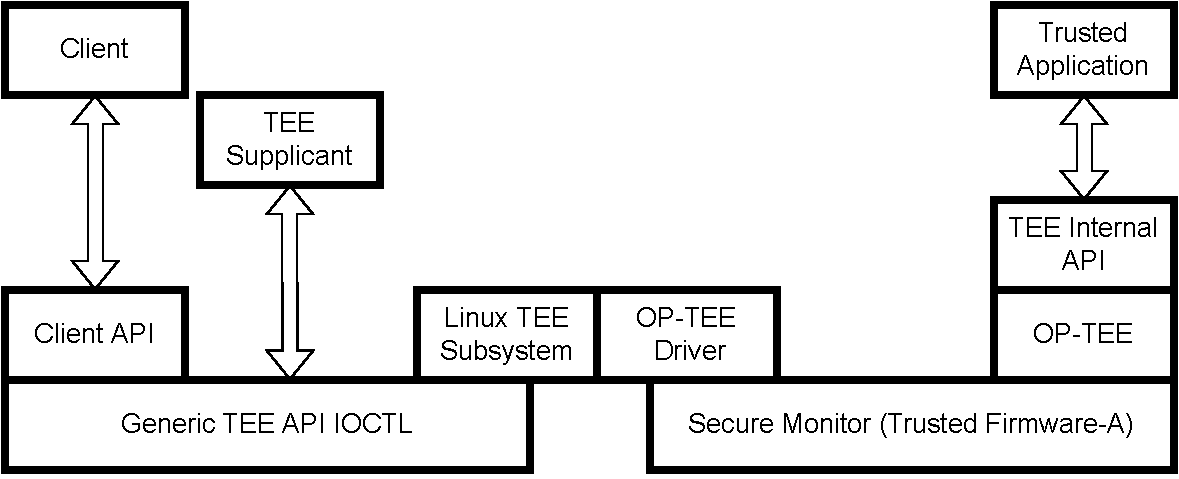
\includegraphics[width=0.8\textwidth]{immagini/optee-system-architecture}
    \caption{
        Architettura software di OP-TEE.
        Da \textit{"TEE Subsystem - OP-TEE Driver"}\cite{linux_tee_subsystem}
    }
    \label{fig:optee-system-architecture}
\end{figure}

OP-TEE include un supporto sperimentale alla virtualizzazione
\cite{optee_virtualization}: in questo
modello è possibile creare dei gruppi di TA isolate dal resto del TEE,
dove ognuno di questi gruppi rappresenta il TEE di una VM.
Questo modello però comporta delle limitazioni, la principale è che,
per evitare un attacco di tipo Denial of Service (DoS), OP-TEE impedisce
un uso dinamico della memoria alle TA, a cui viene assegnata una quantità
di memoria prefissata, statica e uguale per tutti.

Per questi motivi OP-TEE è stato scelto come TEE da utilizzare
come riferimento per la realizzazione del nostro progetto, è
importante però notare che, nonostante ciò, l'implementazione realizzata
non è legata a OP-TEE in particolare, e dovrebbe funzionare con qualsiasi
TEE disponibile nel kernel Linux.

\section{Implementazione}
\label{sec:implementazione}
Il nostro obiettivo è quello di implementare un passthrough per il TEE,
cioè un sistema tramite la quale una macchina virtuale possa mandare
richieste al TEE presente sulla macchina che la ospita, cioè l'host.
Per fare questo abbiamo bisogno di un modo per comunicare tra la macchina
virtuale e l'host, dunque di creare un canale di comunicazione tra i due
mondi e dedicato al TEE.

Nella pratica, creare questo canale di comunicazione vuol dire estendere
l'hypervisor (nel nostro caso QEMU) con un nuovo device virtuale, che sarà
il nostro passthrough.
Aggiungere un nuovo dispositivo implica anche scrivere un driver per
questo device, driver che verrà utilizzato nella sistema guest.

Questo driver si interfaccia con il sottosistema TEE e il device virtuale,
il suo compito dunque è quello di soddisfare le richieste verso il TEE
inoltrando e ricevendo le richieste dal device virtuale.

Host e macchina virtuale comunicano utilizzando questo device e implementano
un semplice protocollo di comunicazione a messaggi; questi messaggi
riflettono le richieste che il guest può fare al TEE. 

\subsection{Device virtuale}
Il device virtuale è stato implementato estendendo la macchina ARM
\texttt{qemu\_virt\_8}. 

La scelta di questo sistema è stata fatta semplicemente perché è
la scelta di default su QEMU, nulla dovrebbe impedire di rendere
accessibile il device virtuale anche ad altre piattaforme e su altre
architetture.

\bigbreak \noindent

Il device comunica con il driver tramite MMIO\footnote{
    Memory Mapped Input/Output
}:
scritture da parte del guest nella zona di memoria
\texttt{0x0b000000}-\texttt{0x0b000200}
passano il controllo dalla VM all'hypervisor, che prende il controllo e
permette di inoltrare il messaggio scritto dal guest.

Questa zona di memoria è suddivisa in registri, che sono utilizzati
per implementare un semplice protocollo a messaggi che imita il funzionamento
dell'interfaccia user-space del sottosistema TEE di Linux.
I registri che abbiamo definito sono:

\begin{table}
    \centering
    \begin{tabular}{|c|c|c|}
        \hline
        \textbf{Registro}   & \textbf{Offset} & \textbf{Dimensione} \\
        \hline
        OPEN\_TEE           & 0x0             & 8 byte \\
        CLOSE\_TEE          & 0x8             & 8 byte \\
        STATUS              & 0x10            & 8 byte \\
        COMMAND\_PTR        & 0x18            & 8 byte \\
        SEND\_COMMAND       & 0x20            & 4 byte \\
        \hline
    \end{tabular}
    \caption{
        Registri del device virtuale di passthrough.
        L'offset è relativo all'inizio della zona di MMIO del device virtuale
    }
    \label{table:registri-device}
\end{table}

In \ref{subsec:interfaccia-user-space} abbiamo descritto nel dettaglio
come l'interfaccia user-space del sottosistema TEE di Linux funziona.
In breve, un programma apre il device file del TEE, effettua delle
\textit{ioctl} e poi lo chiude.

L'uso del device virtuale assomiglia molto a questo processo.
Per esempio, il driver che vuole aprire una nuova connessione con il TEE
legge un valore dal registro \texttt{OPEN\_TEE}.
Il valore letto, se diverso da zero, rappresenta un identificativo
della connessione con una semantica simile a quella dei descrittori
di file.

Per effettuare l'equivalente di una \textit{ioctl}, il driver
prepara un messaggio in un buffer di memoria e scrive l'indirizzo
fisico del messaggio nel registro \texttt{COMMAND\_PTR}.
Infine, scrive un valore qualsiasi di quattro byte sul registro
\texttt{SEND\_COMMAND}.

Dopo ogni operazione, il driver può leggere il registro \texttt{STATUS}
per ottenere informazioni sul successo o fallimento della richiesta.
Inoltre, lo stato dei registri(eccetto \texttt{STATUS}) viene azzerato.

\bigbreak \noindent

L'uso del registro \texttt{SEND\_COMMAND} può sembrare strano,
effettivamente sarebbe più semplice avviare l'operazione con la
scrittura dell'indirizzo nel registro \texttt{COMMAND\_PTR}.
Il problema di questa scelta è che non è sempre possibile effettuare
una scrittura in memoria da otto byte in modo atomico su tutte le
architetture.

Il rischio è dunque che un processore scriva solamente la prima metà
dell'indirizzo, attivando l'hypervisor e facendo iniziare l'operazione
con un indirizzo non valido.

Per questo motivo è stato scelto di utilizzare un registro extra, che
ha il solo scopo di confermare la conclusione la scrittura dell'indirizzo
nel registro \texttt{COMMAND\_PTR}.

\subsection{Driver}
\label{subsection:driver}
Il driver è stato implementato come modulo kernel per Linux, compilato
\textit{out-of-tree}.
Questo implementa il set minimo di funzioni necessarie per integrarsi con
il sottosistema TEE di Linux.

Il driver al caricamento chiama la funzione \texttt{ioremap} per ri-mappare
l'area di memoria del device virtuale in una zona di memoria virtuale
accessibile dal kernel.

In generale, il driver non è particolarmente complesso.
Il suo compito è quello di ricevere delle richieste dal sottosistema TEE
di Linux, convertirle in messaggi compatibili con il protocollo descritto
più avanti, e infine mandare questi messaggi al device virtuale.

Durante l'invio dei messaggi, il driver deve fare attenzione a utilizzare
meccanismi di sincronizzazione, come un semplice lock, per evitare che due
richieste separate al TEE possano interferire tra di loro mentre stanno
provando a comunicare con il device virtuale.

\subsection{Protocollo}
\label{subsection:protocollo}
Il protocollo di comunicazione tra host e guest è molto semplice, ed è
stato progettato per essere il più possibile simile alle operazioni
supportate dai device file TEE reali.

Il protocollo è basato su un sistema a messaggi. Ogni messaggio inizia
con una struttura comune che permette al destinatario di capire come
interpretare il resto del messaggio, raffigurata in
\figurename~\ref{fig:message-wrapper-schema}.

\begin{figure}[H]
    \centering
    \GeneraSchemaPacchetto{
        type/8}{
        payload\_size/8,
        payload/variabile
    }
    \caption{
        Header iniziale di tutti i messaggi del protocollo.
        Questi valori permettono al destinatario di capire come interpretare
        il resto del messaggio, contenuto del payload
    }
    \label{fig:message-wrapper-schema}
\end{figure}

Il campo \texttt{type} permette di identificare come interpretare il
contenuto di \texttt{payload}, questo valore deve dunque essere uno di quelli
descritti più avanti nei corrispondenti messaggi.
Dato che alcuni messaggi possono contenere un numero variabile
(ma comunque limitato) di argomenti, il campo \texttt{payload\_size} indica
la dimensione in byte del campo \texttt{payload} seguente.

In base al tipo di messaggio inviato esistono dei vincoli sui valori
accettabili per il campo \texttt{payload\_size}.
Questi vincoli sono descritti in \tablename~\ref{tab:dimensioni-valide-payload}.

\begin{table}
    \centering
    \begin{tabular}{|m{5.3cm}|c|c|}
        \hline
        \textbf{Comando}    & \textbf{Dimensione Payload} & \textbf{Vincoli}    \\
        \hline
        \texttt{GetVersion}                             & $12$ byte                 & \_                     \\
        \texttt{OpenSession}                            & $64 \leq x \leq 192$ byte & $(x - 64) \mod 32 = 0$ \\
        \texttt{InvokeFunction}                         & $32 \leq x \leq 160$ byte & $(x - 32) \mod 32 = 0$ \\
        \texttt{CancelRequest}                          & $16$ byte                 & \_                     \\
        \texttt{CloseSession}                           & $12$ byte                 & \_                     \\
        \texttt{EnsureMemoryBuffers-AreSynchronized}    & $12 \leq x \leq 112$ byte & $(x - 12) \mod 24 = 0$ \\
        \texttt{FreeSharedMemoryBuffer}                 & $16$ byte                 & \_                     \\
        \hline
    \end{tabular}
    \caption{
        Dimensioni e vincoli sulla dimensione dei payload per i vari messaggi
    }
    \label{tab:dimensioni-valide-payload}
\end{table}

Oltre a un valore di ritorno, leggibile tramite un registro del device
virtuale, il destinatario può anche modificare il contenuto del campo
\texttt{payload} del messaggio, in base al tipo di messaggio inviato.

In generale questi messaggi sono molto simili (ma non uguali) alle strutture
dati definite dall'interfaccia user-space del sottosistema TEE, con delle
aggiunte per aiutare l'hypervisor e per allineare i dati ai 16 byte.

Una modifica condivisa da molti messaggi è il campo \texttt{fd}
(\textit{File Descriptor}). Questo campo ha una semantica simile a quella
dei file descriptor in Linux, seppur in questo caso serva al driver per
decidere a quale connessione aperta tra hypervisor e TEE inoltrare il messaggio.

Un valore \texttt{fd} valido è un valore maggiore o uguale a zero, letto
tramite il registro \texttt{OPEN} del device virtuale.
Messaggi che fanno parte della stessa connessione devono avere
lo stesso valore di \texttt{fd}.

\bigbreak \noindent

Un messaggio in particolare non ha corrispondenza con alcuna \textit{ioctl},
questo è \texttt{EnsureMemoryBuffersAreSynchronized}.
Questo messaggio invia all'hypervisor delle informazioni riguardo alcuni
buffer di memoria condivisi, in particolare il loro ID
(unico all'interno del guest), la loro dimensione allocata e
l'indirizzo fisico in cui si trovano.
Questo messaggio è inviato dal driver prima di inviare un altro messaggio
che fa riferimento a questi buffer, ciò è necessario per assicurarsi
che l'hypervisor possa decidere il corrispondente buffer di memoria
dentro al TEE.
Questo problema è descritto più nel dettaglio in \ref{subsection:hypervisor}.

\paragraph{GetVersion}:

\begin{figure}[H]
    \centering
    \GeneraSchemaPacchetto {impl\_id/4}{impl\_caps/4, gen\_caps/4}
    \caption{Schema del payload di un messaggio \texttt{GetVersion}}
    \label{fig:msg-schema-getversion}
\end{figure} 

Il messaggio \texttt{GetVersion} è identificato da \texttt{type} uguale a
$0$ ed è il messaggio più semplice tra quelli presenti.
Il mittente prepara un payload di dimensione $16$ byte tutti a zero e lo
manda al destinatario, che si occuperà di riempire il payload con le
informazioni riguardo al TEE.
I valori ritornati non sono garantiti essere gli stessi che si ottengono 
tramite la chiamata \textit{ioctl} \texttt{TEE\_IOC\_VERSION} del
sottosistema TEE, questo perché non è garantito che il passthrough
possa supportare tutte le funzionalità extra offerte dal TEE.

Ad esempio, la nostra implementazione non supporta
(banalmente perchè non implementata)
l'uso dei \textit{registered shared memory buffers}, cioè la possibilità per
un client di "promuovere" un buffer allocato normalmente a buffer di memoria
condivisa con il TEE.
Per questo motivo, un client interno a una VM che chiede informazioni riguardo
al TEE leggerà sempre il bit \texttt{TEE\_GEN\_CAP\_REG\_MEM} di
\texttt{gen\_caps} a zero, anche se il TEE fisico in realtà supporta la
funzionalità.

\paragraph{OpenSession, InvokeFunction, CancelRequest e CloseSession}: \\
\begin{figure}[H]
    \centering
    \resizebox{\textwidth}{!}{
    \GeneraSchemaPacchetto {
        fd/8}{
        uuid/16, 
        clnt\_uuid/16, 
        clnt\_login/4, 
        cancel\_id/4, 
        session/4,
        ret/4, 
        ret\_origin/4, 
        num\_params/4, 
        params/variabile
    }}
    \caption{Schema del payload di un messaggio \texttt{OpenSession}}
    \label{fig:msg-schema-opensession}
\end{figure}

\begin{figure}[H]
    \centering
    \resizebox{\textwidth}{!}{
    \GeneraSchemaPacchetto{
        fd/8}{
        func/4, 
        session/4, 
        cancel\_id/4, 
        ret/4, 
        ret\_origin/4, 
        num\_params/4, 
        params/variabile
    }}
    \caption{Schema del payload di un messaggio \texttt{InvokeFunction}}
    \label{fig:msg-schema-invokefunction}
\end{figure}

\begin{figure}[H]
    \centering
    \GeneraSchemaPacchetto{
        fd/4}{
        cancel\_id/4, 
        session/4
    }
    \caption{Schema del payload di un messaggio \texttt{CancelRequest}}
    \label{fig:msg-schema-cancelrequest}
\end{figure}

\begin{figure}[h]
    \centering
    \GeneraSchemaPacchetto{fd/4}{
        session/4
    }
    \caption{Schema del payload di un messaggio \texttt{CloseSession}}
    \label{fig:msg-schema-closesession}
\end{figure}

I messaggi \textit{OpenSession}, \textit{InvokeFunction},
\textit{CancelRequest} e \textit{CloseSession} sono identificati
rispettivamente dai valori \texttt{type} uguale a $2, 3, 4$ e $5$.
Il loro funzionamento e la semantica dei campi è identica a quella delle
rispettive \textit{ioctl} dell'interfaccia user-space del sottosistema TEE
con lo stesso nome.

In aggiunta ai campi delle \textit{ioctl} del sottosistema TEE, troviamo anche
campo extra \texttt{fd} che serve per identificare a quale connessione con
il TEE vogliamo inoltrare il messaggio.
Questo valore è ottenuto dal driver tramite il registro \texttt{OPEN} del
device virtuale; messaggi che fanno parte della stessa connessione dovrebbero
avere lo stesso valore di \texttt{fd}.

La presenza di parametri in numero variabile è l'origine dei vincoli
sulla lunghezza del payload, descritti in
\tablename~\ref{tab:dimensioni-valide-payload}.
Questi vincoli verificano semplicemente che, oltre ai campi della
richiesta, ci siano al massimo quattro parametri per la richiesta e siano
tutti di dimensione 16 byte.

I parametri sono rappresentati alla fine del messaggio, ognuno come tupla
di quattro interi a 64 bit.
La semantica di questi valori è la stessa del sottosistema TEE, cioè il
primo di questi interi definisce il tipo dell'argomento e gli
altri tre sono dei valori dipendenti dal tipo.

Se un parametro è di tipo \textit{memref}, cioè è un buffer di memoria
condivisa con il TEE, è necessario che, prima del suo utilizzo, il client
lo abbia segnalato all'hypervisor tramite il messaggio
\textit{EnsureMemoryBuffersAreSynchronized}.

\paragraph{EnsureMemoryBuffersAreSynchronized}: \\
\begin{figure}[H]
    \centering
    \GeneraSchemaPacchetto{
        fd/8}{
        num\_buffers/4,
        buffer/variabile
    }
    \caption{
        Schema del payload di un messaggio
        \texttt{EnsureMemoryBuffersAreSynchronized}}
    \label{fig:msg-schema-embas}
\end{figure}
Il messaggio \textit{EnsureMemoryBuffersAreSynchronized} è identificato da
\texttt{type} uguale a $5$ ed è utilizzato per segnalare all'hypervisor
l'ID locale di un buffer di memoria condivisa all'hypervisor.

Questa operazione non ha una equivalente \textit{ioctl} ed è necessaria
per l'implementazione del passthrough.
Ogni buffer di memoria condivisa con il TEE è identificato con un ID numerico
all'interno del sottosistema TEE.
Questi ID sono assegnati dal sistema operativo, dunque un ID interno a una
macchina virtuale non corrisponde necessariamente allo stesso buffer
all'esterno della VM.

Questo messaggio segnala all'hypervisor l'allocazione di uno o più buffer di
memoria, e l'ID locale corrispondente a tale buffer.
Grazie a queste informazioni l'hypervisor potrà tradurre gli ID locali nei
parametri degli altri messaggi negli ID corretti al di fuori della VM.

Dunque, prima che un buffer allocato venga usato come parametro di una
richiesta,
è necessario che il client abbia inviato almeno un messaggio
\textit{EnsureMemoryBuffersAreSynchronized} con le sue informazioni.

Una discussione più approfondita su questa problematica è data più avanti in
\ref{subsection:hypervisor}.

\paragraph{FreeSharedMemoryBuffer}: \\
\begin{figure}[H]
    \centering
    \GeneraSchemaPacchetto{
        fd/8}{
        buf\_id/8
    }
    \caption{Schema del payload di un messaggio \texttt{FreeSharedMemoryBuffer}}
    \label{fig:msg-schema-freebuf}
\end{figure}
Il messaggio \textit{FreeSharedMemoryBuffer} è identificato da \texttt{type}
uguale a $6$ ed è utilizzato liberare la memoria condivisa allocata
precedentemente.

Questa operazione non ha una equivalente \textit{ioctl}, questo perchè
nell'interfaccia user-space del sottosistema TEE la deallocazione di un
buffer di memoria corrisponde al momento in cui il client chiude il
descrittore del file associato al buffer.

I due parametri rappresentano rispettivamente la connessione con il TEE
e l'ID (locale al guest) del buffer di memoria da liberare.

\subsection{Hypervisor}
\label{subsection:hypervisor}
Il lato dell'hypervisor è dove si nasconde la parte più complessa del progetto.

L'hypervisor deve, per prima cosa, implementare il device virtuale.
Per fare ciò, mantiene uno "stato" dei registri che viene aggiornato a ogni
scrittura da parte del guest nella zona di MMIO del device.
Una scrittura all'offset del registro \texttt{SEND\_COMMAND} indica il momento
in cui l'hypervisor deve gestire un messaggio del protocollo.

Implementare la maggior parte dei messaggi del protocollo è concettualmente
semplice, dato che hanno spesso una corrispondenza diretta con una
\textit{ioctl}.
Ad alto livello, uno dei ruoli dell'hypervisor è quello di ricevere
i messaggi, fare le rispettive \textit{ioctl} e riscrivere nella memoria
dell'host il risultato.

Il problema principale è che i dati passati dal guest all'hypervisor sono
valori validi solo all'interno della VM. Eseguire una \textit{ioctl}
usando direttamente quei valori non funzionerebbe.

Un esempio di questo problema sono i descrittori di file utilizzati nella
chiamata \textit{ioctl}: 
il descrittore di file che una VM possiede per accedere al device file del TEE
non è lo stesso valore con cui l'hypervisor può fare una \textit{ioctl},
è necessario mantenere una tabella di traduzioni tra questi valori e
utilizzare il valore adatto al mondo in cui ci si trova.

Un secondo esempio di un problema simile, ma più complesso, è la gestione
dell'allocazione dei buffer di memoria condivisa con il TEE.
Ogni buffer è identificato da un ID numerico, che viene assegnato dal sistema
operativo, dunque lo stesso buffer è identificato da valori diversi dentro
e fuori la VM.

Anche in questo caso è necessario dunque mantenere una tabella di traduzioni
tra questi valori e tradurre gli ID presenti nei messaggi prima di inoltrarli
all'altro mondo.

Costruire questa tabella delle traduzioni degli ID per i buffer di memoria è
più difficile rispetto a quella dei descrittori di file.
Il motivo è dato da un dettaglio tecnico del sottosistema TEE di Linux, che
assegna un ID solamente quando la funzione di allocazione di memoria del driver
ha restituito un buffer.
Questo crea una dipendenza circolare, dove per allocare un buffer
abbiamo bisogno di un ID, ma per ottenere un ID abbiamo bisogno di
allocare prima il buffer.

Modificare il kernel Linux è una soluzione che potrebbe risolvere il problema
in modo pulito, ma uno dei nostri obiettivi è quello di mantenere il kernel
invariato e di integrare la nostra implementazione come un TEE normale. 

Per risolvere questo problema semplicemente decidiamo di rimandare
l'allocazione
al primo utilizzo del buffer come parametro di una operazione.
Questo è il vero scopo del messaggio
\textit{EnsureMemoryBuffersAreSynchronized},
permettere di ritardare la vera allocazione del buffer sottostante e
di soddisfarla solo quando è necessaria.

\bigbreak \noindent

Una volta che abbiamo risolto questi due problemi, rimane il problema di
come rendere questi buffer di memoria effettivamente "condivisi" tra TEE
e guest.
I buffer allocati dall'hypervisor con il TEE sono effettivamente condivisi,
ma sarebbe necessario condividere questa memoria anche con il guest.

Fare questo è possibile, ma richiede delle modifiche sostanziali a QEMU, per
questo motivo abbiamo scelto una strada molto più semplice, seppur
inefficiente.

Lo standard GlobalPlatform riconosce che non sempre è possibile implementare
un meccanismo di memoria condivisa, condividendo la vera memoria fisica,
cioè senza copie.
In queste situazioni la soluzione è quella di mantenere due buffer di memoria
diversi, ma di uguali dimensioni, uno per il TEE e uno per il REE.
Questi buffer vengono sincronizzati tramite una copia dei dati da uno all'altro
ogni volta che si raggiunge un \textit{punto di sincronizzazione}.

\begin{figure}[h]
    \centering
    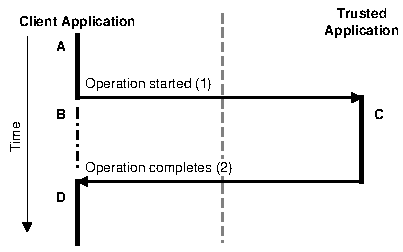
\includegraphics{immagini/tp-synchronization-points}
    \caption{
        Punti di sincronizzazione buffer di memoria condivisa.
        Da \textit{
            3.2.5 Memory References GlobalPlatform TEE Client Specification
        }
    }
    \label{fig:gp-punti-sincronizzazione}
\end{figure}

Questi \textit{punti di sincronizzazione}, raffigurati in
\figurename~\ref{fig:gp-punti-sincronizzazione} delle specifiche GlobalPlatform,
sono banalmente i momenti in cui si attraversa la barriera tra TEE e REE.

Nel nostro caso, però, abbiamo due barriere: una tra TEE e hypervisor,
che funziona
senza dover far nulla, e una tra hypervisor e VM, che dobbiamo implementare.
Implementare la sincronizzazione è solamente questione di copiare i dati dal
guest al buffer accessibile all'hypervisor prima di iniziare una chiamata
al TEE, e fare l'opposto (cioè da buffer dell'hypervisor a buffer locale
del guest) prima di ritornare il controllo alla VM.

Questa è una soluzione piuttosto inefficiente, ma funzionale per lo scopo di
prototipazione.

\section{Verifica funzionale e performance}
\label{sec:verifica-funzionale-e-performance}
Lo sviluppo e la verifica del prototipo è stata fatta utilizzando una macchina
virtuale QEMU simulando una macchina virtuale ARMv8 con supporto a TrustZone,
un processore Cortex-A72 con 2 core e 1GB di RAM.
Su questa VM abbiamo installato Linux versione 5.19.0,
Busybox 1.34.1 compilato tramite Buildroot e, come TEE, OP-TEE versione
3.19.0-ge0cfd556.
Questa VM, che chiameremo VM1, è stata utilizzata per simulare la macchina
host nel nostro prototipo. Infatti, dentro la VM1 abbiamo eseguito una
seconda macchina virtuale utilizzando la nostra versione modificata di QEMU.
Questa VM, che chiameremo VM2, è stata utilizzata per simulare la macchina
guest nel nostro prototipo e simula una macchina ARM \textit{virt} con
processore \textit{"kvm"}, cioè sfruttando le funzionalità di virtualizzazione
del kernel Linux.
Dentro la VM2 abbiamo installato Linux versione 5.15.18 con Busybox 1.35.0
e caricato il nostro driver per il passthrough TEE.
Per verificare la correttezza del nostro prototipo abbiamo usato due set di
test cases.

Il primo set sono i programmi di esempio forniti da OP-TEE: sono piccoli
programmi user-space e Trusted Application a scopo didattico e che testano le
funzionalità offerte dall'interfaccia GlobalPlatform e che fanno uso di
\textit{libteec} per comunicare con il TEE, una libreria wrapper
dell'interfaccia user-space del sottosistema TEE di Linux.
Questi programmi includono il classico "Hello World", una implementazione
dell'algoritmo AES, un programma che salva e recupera dati dallo storage
sicuro offerto dal TEE, un programma che genera blocchi di dati
sfruttando il generatore sicuro di dati random di OP-TEE e altri
programmi che utilizzano funzionalità specifiche di OP-TEE.
Questi piccoli programmi, seppur utilizzino tutte le feature dell'interfaccia
TEE e siano stati di aiuto durante lo sviluppo del prototipo, chiaramente
hanno un utilizzo limitato per la verifica funzionale del prototipo.

Il secondo set è la suite \textit{xtest}, un insieme di poco meno di
$10000$ test sviluppati dal progetto OP-TEE. 
Questa suite nasce per testare le funzionalità di OP-TEE, ma utilizzando
l'interfaccia del sottosistema TEE di Linux la gran parte dei test è
applicabile a qualunque TEE che implementi un driver Linux. 
Su XXXX test, solamente XXX falliscono, ma questi sono tutti test che
fanno uso di funzionalità specifiche di OP-TEE che sono al di fuori
dell'interfaccia TEE standard e dunque fuori dallo scopo del nostro
progetto.

Infine, abbiamo inoltre effettuato dei semplici test delle performance,
nonostante ribadiamo che la nostra implementazione sia intenzionalmente
primitiva e inefficiente.
Per misurare le performance abbiamo usato il comando Unix \textit{time}
eseguendo l'intera suite di test \textit{xtest}.
Noi siamo interessati all'overhead del passthrough, dunque leggeremo la
misura \textit{"sys"}, che indica il tempo speso in kernel mode dal computer
per servire un processo. 

Abbiamo eseguito le misure 10 volte e i risultati sono riportati
in \tablename~\ref{tab:performance}.
A confronto abbiamo anche riportato i tempi di esecuzione ottenuti ripetendo
lo stesso test eseguendo direttamente i test case sulla VM host
(cioè la VM esterna), che accede direttamente al TEE senza passare dal
nostro passthrough.

\begin{table}[ht]
    \centering
    \begin{tabular}{|c|c|c|c|c|c|c|c|c|c|c|c|}
        \hline
        \textbf{Test} & 1 & 2 & 3 & 4 & 5 & 6 & 7 & 8 & 9 & 10 & \textbf{Media} \\
        \hline
        \textbf{Base} & x & x & x & x & x & x & x & x & x & x  & \textbf{x} \\
        \hline
        \textbf{Passthrough} & x & x & x & x & x & x & x & x & x & x & \textbf{x} \\
        \hline
        \textbf{Overhead} & x & x & x & x & x & x & x & x & x & x & \textbf{x} \\
        \hline
    \end{tabular}
    \label{tab:performance}
    \caption{
        Confronto tra tempi di esecuzione con e senza passthrough su
        tutti i test di \textit{xtest}.
    }
\end{table}

Chiaramente i tempi di esecuzione utilizzando il passthrough sono più alti.
Il sospetto è che questo sia dovuto principalmente per l'implementazione
inefficiente della sincronizzazione dei buffer di memoria condivisa.
Infatti, se dividiamo i test case in due categorie, quelli che fanno
uso di memoria condivisa e quelli che non lo fanno, e ripetiamo i test
(riportati in \tablename~\ref{tab:performance-no-shmem}) si nota che
i tempi di esecuzione sono dei secondi sono molto simili ai tempi
senza passthrough.

\begin{table}
    \centering
    \begin{tabular}{|c|c|c|c|c|c|c|c|c|c|c|c|}
        \hline
        \textbf{Test} & 1 & 2 & 3 & 4 & 5 & 6 & 7 & 8 & 9 & 10 & \textbf{Media} \\
        \hline
        \textbf{Base} & x & x & x & x & x & x & x & x & x & x  & \textbf{x} \\
        \hline
        \textbf{Passthrough} & x & x & x & x & x & x & x & x & x & x & \textbf{x} \\
        \hline
        \textbf{Overhead} & x & x & x & x & x & x & x & x & x & x & \textbf{x} \\
        \hline
    \end{tabular}
    \label{tab:performance-no-shmem}
    \caption{
       Confronto tra tempi di esecuzione con e senza passthrough solo
       sui test di \textit{xtest} che non usano shared memory.
    }
\end{table}

L'uso di test case per confrontare le performance non necessariamente
riflette dei carichi di lavoro reali, ma è un modo semplice per avere
un'idea delle prestazioni.

\chapter{Conclusioni}
\label{chap:conclusioni}
In questa tesi abbiamo presentato una possibile soluzione per l'uso dei
Trusted Execution Environment (TEE) in ambienti virtualizzati.
I TEE sono ambienti di computazione integrati nel processore principale
che permettono di garantire diverse proprietà di sicurezza per le
applicazioni eseguite al loro interno.

L'interesse verso il loro uso in ambienti virtualizzati è constatato dalla
fondazione della Confidential Computing Consortium.
Le soluzioni al momento sul mercato richiedono ai clienti di portare con sé
un TEE con le loro applicazioni; questa è una soluzione flessibile ma che
porta con se alcuni limiti tecnici per poterne garantire la sicurezza
e un grande lock-in rispetto alla tecnologia usata.

La soluzione proposta in questa tesi utilizza un approccio diverso che
permette di evitare questi limiti ed è agnostica al TEE e all'architettura
sottostante:
invece di dover portare con sé un TEE, i clienti possono utilizzarne uno
configurato dal vendor con una serie di servizi preinstallati.

La nostra proposta non è in conflitto con quelle già presenti sul mercato;
questo crea un tradeoff interessante per i clienti che possono scegliere
se gestire un TEE da soli, con tutti i vantaggi e svantaggi che ne derivano,
oppure utilizzare un TEE preconfigurato dal vendor, con un lock-in minore
ma con meno flessibilità.

Abbiamo dimostrato la fattibilità del nostro approccio tramite un prototipo,
implementato modificando l'hypervisor QEMU e il sistema operativo Linux.
Infine abbiamo messo alla prova la nostra implementazione tramite la test
suite \textit{xtest} e il TEE \textit{OP-TEE}.

Le performance del nostro prototipo non sono entusiasmanti, seppur accettabili
in molti casi, ma queste sono causate dalla banalità dell'implementazione e
non da limitazioni intrinseche del nostro approccio.
Riteniamo dunque che, seppur sia necessario ancora del lavoro per rendere
l'implementazione utilizzabile in pratica, il nostro approccio sia un buon
punto di partenza

\section{Sviluppi futuri}
\label{sec:sviluppi-futuri}
Il nostro lavoro trascura alcuni aspetti che potrebbero essere interessanti
in base al contesto in cui si vuole utilizzare la nostra soluzione.

Come detto in precedenza, la nostra implementazione trascura le performance in
favore di una implementazione semplice e facile da comprendere.
Questo è un aspetto che potrebbe essere migliorato in futuro, per esempio
implementando il meccanismo dei \textit{Registered Shared Memory Buffers},
che permette di ridurre le allocazioni di memoria.

Inoltre, seppur non strettamente necessarie secondo gli standard GlobalPlatform,
il sottosistema Linux supporta delle funzionalità extra che, in alcuni casi,
potrebbero essere utili per implementare ottimizzazioni.

\bigbreak \noindent

Una limitazione significativa della nostra implementazione attuale è data dalle
periferiche \textit{trusted}: al momento non è presente alcun meccanismo per
permettere la virtualizzazione di queste periferiche all'interno della VM.
Potrebbe essere interessante studiare come permettere la virtualizzazione
di queste periferiche, senza comprometterne la sicurezza.

\bigbreak \noindent

Infine, in ambito cloud computing, una sfida interessante è quella di permettere
il trasferimento di una VM che fa uso di un TEE da un server fisico ad un altro.
Per design, i dati salvati dentro un TEE sono legati strettamente alle chiavi
dentro esso, e quindi non possono essere trasferiti direttamente da un
server ad un altro.
Esplorare come realizzare questo spostamento,
in modo sicuro e trasparente per l'utente, potrebbe essere una direzione di ricerca.

\appendix
\chapter{FakeTEE: Simulatore di TEE per lo sviluppo}
\label{app:faketee}
Sviluppare applicazioni che utilizzano un Trusted Execution Environment può
essere difficile, non solo per l'attenzione necessaria a non violare
le restrizioni imposte dal TEE, ma anche per l'assenza di un ambiente di
sviluppo che permetta di testare il software in un ambiente controllato.

Come precedentemente discusso nella tesi, la maggior parte dei TEE al giorno
d'oggi non consente di installare applicazioni di terze parti, inoltre
a causa della scarsità di informazioni sulle implementazioni dei TEE
è spesso difficile capire se le interazioni del nostro software con quello
del TEE sono corrette.

L'utilizzo di una macchina virtuale per emulare un sistema provvisto di TEE
riprogrammabile e ispezionabile è una alternativa funzionale, ma
l'esperienza di sviluppo con questa soluzione può essere frustrante per
diversi motivi, tra cui: la necessità di dover gestire un secondo sistema
operativo durante lo sviluppo, dover avviare una macchina virtuale per ogni
test, la necessità di cross-compilare il software per la macchina virtuale
e il dover spostare ripetutamente file tra la macchina virtuale e il sistema
host.

In questo progetto abbiamo sviluppato un modulo del kernel di Linux chiamato
"FakeTEE" per evitare questa strada. FakeTEE si aggancia al sottosistema TEE
di Linux e finge di essere un TEE reale, precaricato con delle
Trusted Application scritte direttamente nel suo codice.

FakeTEE ovviamente non può assolutamente offrire alcuna garanzia di sicurezza
perché non è un TEE reale, ma è utile per lo sviluppo di software che
interagiscono con un TEE, in quanto non solo permette di testare il software
direttamente sul proprio sistema sprovvisto di TEE, ma logga una serie di
informazioni utili al debugging sulla console del sistema.

Il codice di FakeTEE è relativamente semplice e di piccole dimensioni, per
questo motivo è facile da modificare e ricaricare durante lo sviluppo.
Il modulo di default contiene delle semplici Trusted Application per provare
le funzionalità base dell'interfaccia GlobalPlatform.
Queste sono utili per testare funzionalità come il passaggio di parametri o
l'uso di memoria condivisa tra TEE e applicazione, ma possono essere
facilmente modificate o sostituite con altre applicazioni.

\chapter{Impostazione dell'ambiente di sviluppo e testing}
\label{app:impostazione-ambiente-sviluppo-testing}
Questa appendice descrive come impostare un ambiente di sviluppo e testing
per il nostro progetto utilizzando il TEE open-source OP-TEE.
Queste istruzioni assumono che si abbia già clonato tutti i repository
elencati in \ref{app:codice-sorgente}, e che si abbia già compilato OP-TEE e
preparato un ambiente virtualizzato dove è possibile provarlo.
A tale scopo, si consiglia di seguire le istruzioni presenti nella
documentazione di OP-TEE.

Alla fine di queste istruzioni si avrà un ambiente con due macchine virtuali,
una dentro l'altra, dove quella più esterna emula un TEE con OP-TEE, mentre
quella interna contiene un passthrough che gli permette di accedere al TEE
emulato. Sia nella VM esterna, che in quella interna, sarà possibile eseguire
la test suite \texttt{xtest}.

\medbreak

Il primo passo consiste nel compilare la versione modificata di QEMU per
poterla utilizzare dentro la VM che emula il TEE.
Per fare ciò, entrare nella cartella \texttt{qemu-tee-passthrough} e
seguire le istruzioni presenti nella documentazione di QEMU,
stando attenti a installare le librerie necessarie in versione arm64
e utilizzando la stessa toolchain utilizzata da OP-TEE per compilare i
software user-space.

Una volta fatto ciò, serve preparare il sistema Linux da eseguire dentro la
VM interna. Un modo semplice consiste nell'utilizzare Buildroot, uno
strumento per la creazione di immagini Linux personalizzate.
Buildroot contiene una configurazione di default per la macchina "virt"
di QEMU, che è la macchina virtuale che utilizzeremo per eseguire la
VM interna.
Una volta terminato il processo di build, si dovrebbe ottenere un file
\texttt{Image}, cioè il kernel Linux, e un file \texttt{rootfs.ext2} con
l'immagine del file system.

A questo punto, bisogna compilare il driver per il passthrough.
Per farlo, entrare nella cartella \texttt{linux-tee-passthrough-driver}
e lanciare il comando \texttt{make} utilizzando come toolchain la stessa
utilizzata da Buildroot per compilare il sistema al punto precedente.
Per configurare la toolchain da utilizzare è possibile modificare il file
\texttt{Makefile} e impostare le variabili relative.
Una volta terminato, si dovrebbe ottenere un file \texttt{driver.ko}.

Questo driver dovrà essere caricato nella VM interna, dunque è necessario
copiarlo dentro il rootfs appena generato. Per farlo, basta montare l'immagine
\texttt{rootfs.ext2} e copiare il file \texttt{driver.ko} dentro la cartella
\texttt{/root}.

\medbreak

Questi tre file sono i componenti necessari per ottenere un sistema con
passthrough; per compilare anche la test suite \texttt{xtest} è necessario
entrare nella cartella \texttt{optee\_test} e compilarla utilizzando la stessa
toolchain usata al punto precedente.
Alla fine del processo si otterrà un file eseguibile chiamato \texttt{xtest},
che, una volta eseguito, farà partire tutti i test.

\medbreak

Come ultimo passo, bisogna mettere insieme tutti i componenti.
Per fare ciò, creare una cartella nella root di OP-TEE dove verranno condivisi
i file tra la macchina host e la VM esterna.
Dentro questa cartella, copiare i file \texttt{Image}, \texttt{rootfs.ext2}
e la cartella di build di \texttt{qemu-tee-passthrough}.
Seguendo le istruzioni presenti nella documentazione di OP-TEE, lanciare
la VM esterna con i rispettivi flag per abilitare la condivisione della cartella.

\medbreak

Dentro la VM, navigare nella cartella condivisa e lanciare \texttt{qemu-tee-passthrough}
con le opzioni \texttt{-machine virt, -kernel Image, -initrd rootfs.ext2}.
Dentro la VM interna, caricare il driver per il passthrough con \texttt{insmod ./driver.ko}
e infine lanciare \texttt{xtest}.
A questo punto dovrebbero essere eseguiti tutti i test.

\chapter{Codice sorgente}
\label{app:codice-sorgente}
Il codice sorgente del progetto è disponibile su GitHub ai seguenti indirizzi:

\begin{itemize}
    \item 
        \textbf{QEMU con supporto a TEE passthrough}: \\
        \noindent 
        \url{https://github.com/mrkct/qemu-tee-passthrough}
    \item
        \textbf{Driver Linux per TEE passthrough}: \\ 
        \noindent
        \url{https://github.com/mrkct/tee-passthrough-linux-driver}
    \item
        \textbf{FakeTEE}: \\
        \noindent
        \url{https://github.com/mrkct/fake-tee}
\end{itemize}

\bibliographystyle{unsrt}
\bibliography{bibliografia}
\addcontentsline{toc}{chapter}{Bibliografia}

\end{document}
